% Options for packages loaded elsewhere
\PassOptionsToPackage{unicode}{hyperref}
\PassOptionsToPackage{hyphens}{url}
%
\documentclass[
]{article}
\usepackage{amsmath,amssymb}
\usepackage{lmodern}
\usepackage{iftex}
\ifPDFTeX
  \usepackage[T1]{fontenc}
  \usepackage[utf8]{inputenc}
  \usepackage{textcomp} % provide euro and other symbols
\else % if luatex or xetex
  \usepackage{unicode-math}
  \defaultfontfeatures{Scale=MatchLowercase}
  \defaultfontfeatures[\rmfamily]{Ligatures=TeX,Scale=1}
\fi
% Use upquote if available, for straight quotes in verbatim environments
\IfFileExists{upquote.sty}{\usepackage{upquote}}{}
\IfFileExists{microtype.sty}{% use microtype if available
  \usepackage[]{microtype}
  \UseMicrotypeSet[protrusion]{basicmath} % disable protrusion for tt fonts
}{}
\makeatletter
\@ifundefined{KOMAClassName}{% if non-KOMA class
  \IfFileExists{parskip.sty}{%
    \usepackage{parskip}
  }{% else
    \setlength{\parindent}{0pt}
    \setlength{\parskip}{6pt plus 2pt minus 1pt}}
}{% if KOMA class
  \KOMAoptions{parskip=half}}
\makeatother
\usepackage{xcolor}
\IfFileExists{xurl.sty}{\usepackage{xurl}}{} % add URL line breaks if available
\IfFileExists{bookmark.sty}{\usepackage{bookmark}}{\usepackage{hyperref}}
\hypersetup{
  pdftitle={Dixon Woods},
  pdfauthor={Ted Hillert},
  hidelinks,
  pdfcreator={LaTeX via pandoc}}
\urlstyle{same} % disable monospaced font for URLs
\usepackage[margin=1in]{geometry}
\usepackage{longtable,booktabs,array}
\usepackage{calc} % for calculating minipage widths
% Correct order of tables after \paragraph or \subparagraph
\usepackage{etoolbox}
\makeatletter
\patchcmd\longtable{\par}{\if@noskipsec\mbox{}\fi\par}{}{}
\makeatother
% Allow footnotes in longtable head/foot
\IfFileExists{footnotehyper.sty}{\usepackage{footnotehyper}}{\usepackage{footnote}}
\makesavenoteenv{longtable}
\usepackage{graphicx}
\makeatletter
\def\maxwidth{\ifdim\Gin@nat@width>\linewidth\linewidth\else\Gin@nat@width\fi}
\def\maxheight{\ifdim\Gin@nat@height>\textheight\textheight\else\Gin@nat@height\fi}
\makeatother
% Scale images if necessary, so that they will not overflow the page
% margins by default, and it is still possible to overwrite the defaults
% using explicit options in \includegraphics[width, height, ...]{}
\setkeys{Gin}{width=\maxwidth,height=\maxheight,keepaspectratio}
% Set default figure placement to htbp
\makeatletter
\def\fps@figure{htbp}
\makeatother
\setlength{\emergencystretch}{3em} % prevent overfull lines
\providecommand{\tightlist}{%
  \setlength{\itemsep}{0pt}\setlength{\parskip}{0pt}}
\setcounter{secnumdepth}{-\maxdimen} % remove section numbering
\newlength{\cslhangindent}
\setlength{\cslhangindent}{1.5em}
\newlength{\csllabelwidth}
\setlength{\csllabelwidth}{3em}
\newlength{\cslentryspacingunit} % times entry-spacing
\setlength{\cslentryspacingunit}{\parskip}
\newenvironment{CSLReferences}[2] % #1 hanging-ident, #2 entry spacing
 {% don't indent paragraphs
  \setlength{\parindent}{0pt}
  % turn on hanging indent if param 1 is 1
  \ifodd #1
  \let\oldpar\par
  \def\par{\hangindent=\cslhangindent\oldpar}
  \fi
  % set entry spacing
  \setlength{\parskip}{#2\cslentryspacingunit}
 }%
 {}
\usepackage{calc}
\newcommand{\CSLBlock}[1]{#1\hfill\break}
\newcommand{\CSLLeftMargin}[1]{\parbox[t]{\csllabelwidth}{#1}}
\newcommand{\CSLRightInline}[1]{\parbox[t]{\linewidth - \csllabelwidth}{#1}\break}
\newcommand{\CSLIndent}[1]{\hspace{\cslhangindent}#1}
\ifLuaTeX
  \usepackage{selnolig}  % disable illegal ligatures
\fi

\title{Dixon Woods}
\usepackage{etoolbox}
\makeatletter
\providecommand{\subtitle}[1]{% add subtitle to \maketitle
  \apptocmd{\@title}{\par {\large #1 \par}}{}{}
}
\makeatother
\subtitle{Plant species and descriptions.}
\author{Ted Hillert}
\date{}

\begin{document}
\maketitle

{
\setcounter{tocdepth}{2}
\tableofcontents
}
\hypertarget{acer-rubrum}{%
\section{\texorpdfstring{\emph{Acer rubrum}}{Acer rubrum}}\label{acer-rubrum}}

\hypertarget{common-names-carolina-maple-curled-maple-red-maple-scarlet-maple-soft-maple-swamp-maple-and-water-maple}{%
\subsection{Common names; Carolina maple, Curled maple, Red maple, Scarlet maple, Soft maple, Swamp maple, and Water maple}\label{common-names-carolina-maple-curled-maple-red-maple-scarlet-maple-soft-maple-swamp-maple-and-water-maple}}

\begin{figure}

{\centering 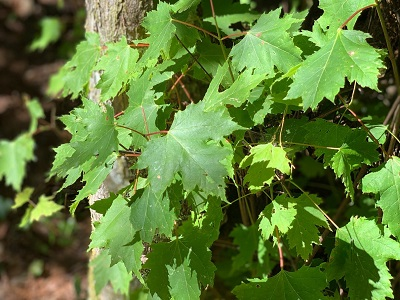
\includegraphics[width=0.5\linewidth]{acer1} 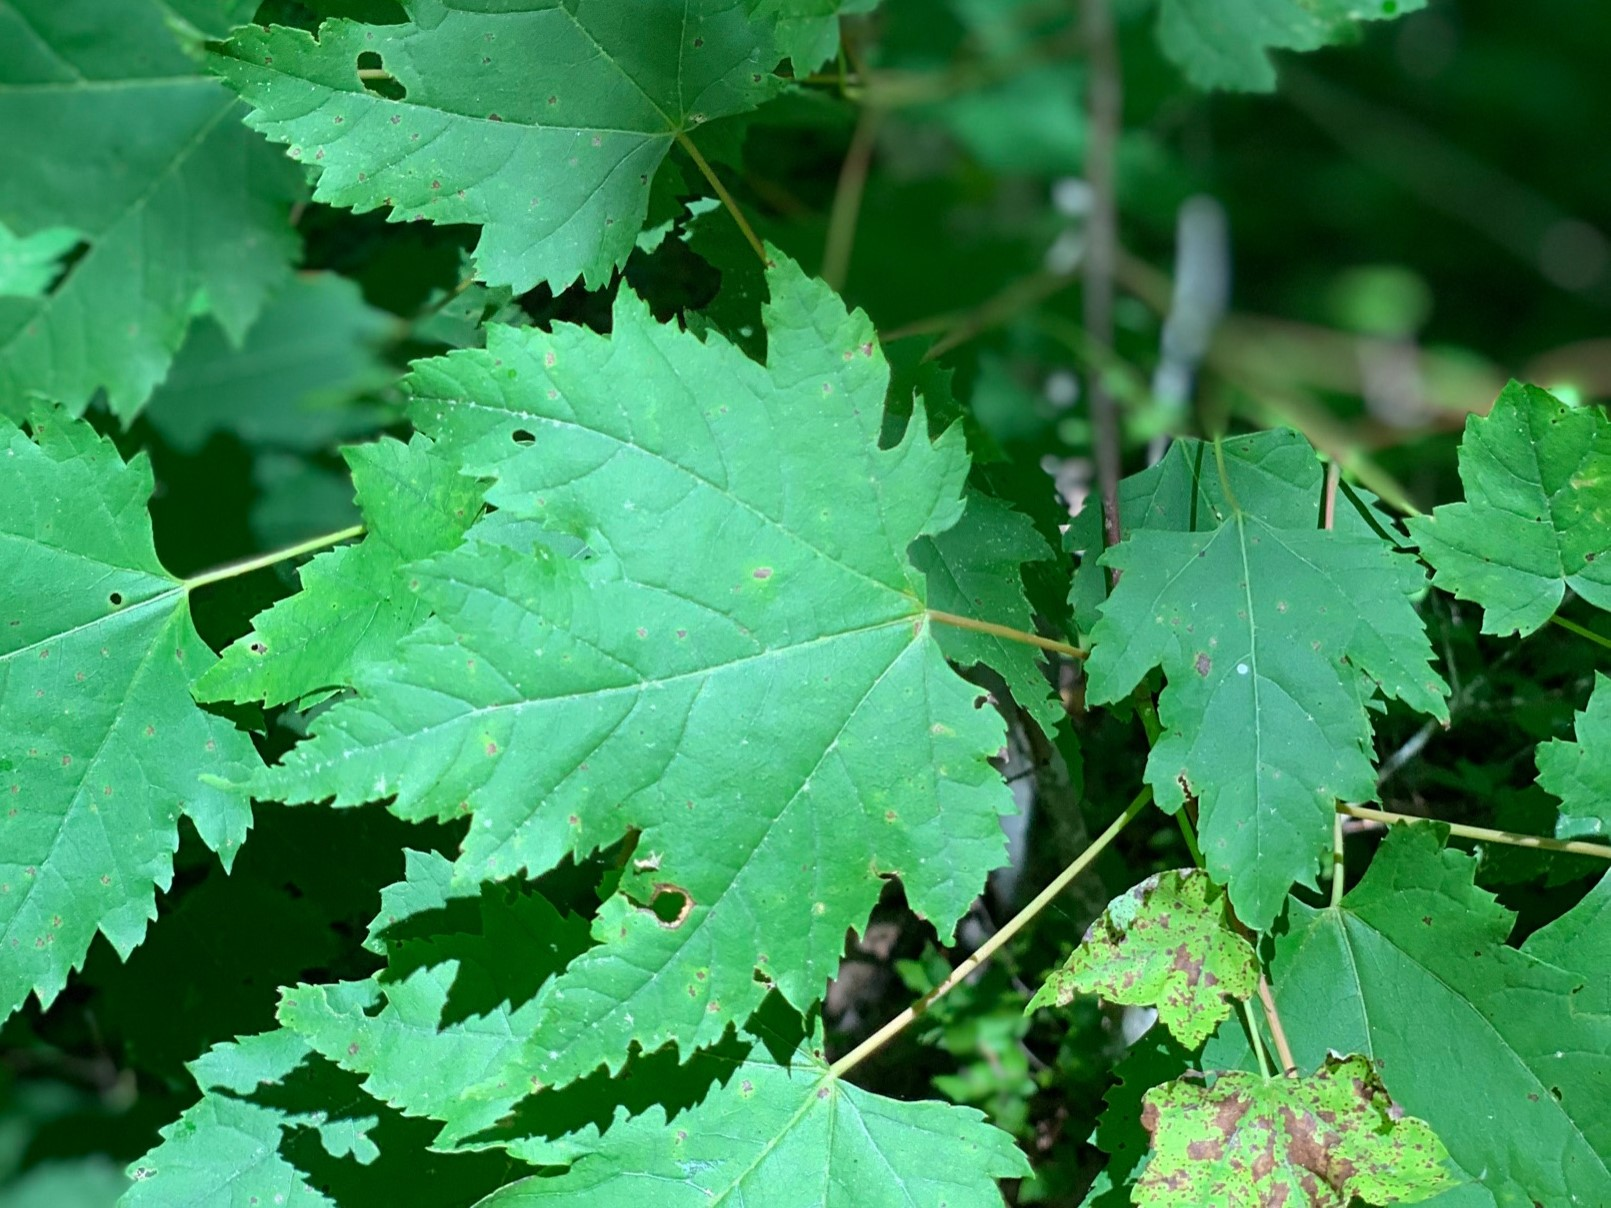
\includegraphics[width=0.5\linewidth]{redmap} 

}

\caption{*Acer rubrum* leaves (left), floral bloom (right) (Illustration courtesy of Patterson Clark).}\label{fig:maple}
\end{figure}

\emph{Acer rubrum} is a perennial deciduous tree in Sapindaceae family (soapberry) that can grow up to 120 feet tall, but more commonly reaches up to 70 feet tall and 2.5 feet in diameter at breast height. This native tree is tolerant of a wide range of soils but prefers slightly acidic, moist and well-draining soil in partial shade to full sun. It is a cold tolerant tree that is fast-growing than Norway and Sugar maples but slower than Silver maple. The leaves of this maple are palmate (hand-shaped), lobed with serrate (toothed) margins, and a rounded cordate (heart-shaped) base. They are arranged opposite each other and will turn red or yellow in fall, also being some of the first trees to turn color. Red maples will flower once in the Spring and again in Winter, with the male trees displaying decorative red blooms. (TWC and GDG 2015, NCSU n.d.a)

Further reading; \href{https://plants.ces.ncsu.edu/plants/acer-rubrum/}{\emph{Acer rubrum}}, \href{https://www.wildflower.org/plants/result.php?id_plant=acru}{\emph{Acer rubrum}}

\hypertarget{castanea-dentata}{%
\section{\texorpdfstring{\emph{Castanea dentata}}{Castanea dentata}}\label{castanea-dentata}}

\hypertarget{common-names-american-chestnut-and-chestnut}{%
\subsection{Common names; American Chestnut and Chestnut}\label{common-names-american-chestnut-and-chestnut}}

\begin{figure}

{\centering 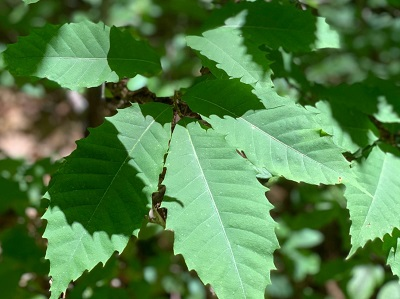
\includegraphics[width=0.5\linewidth]{castden} 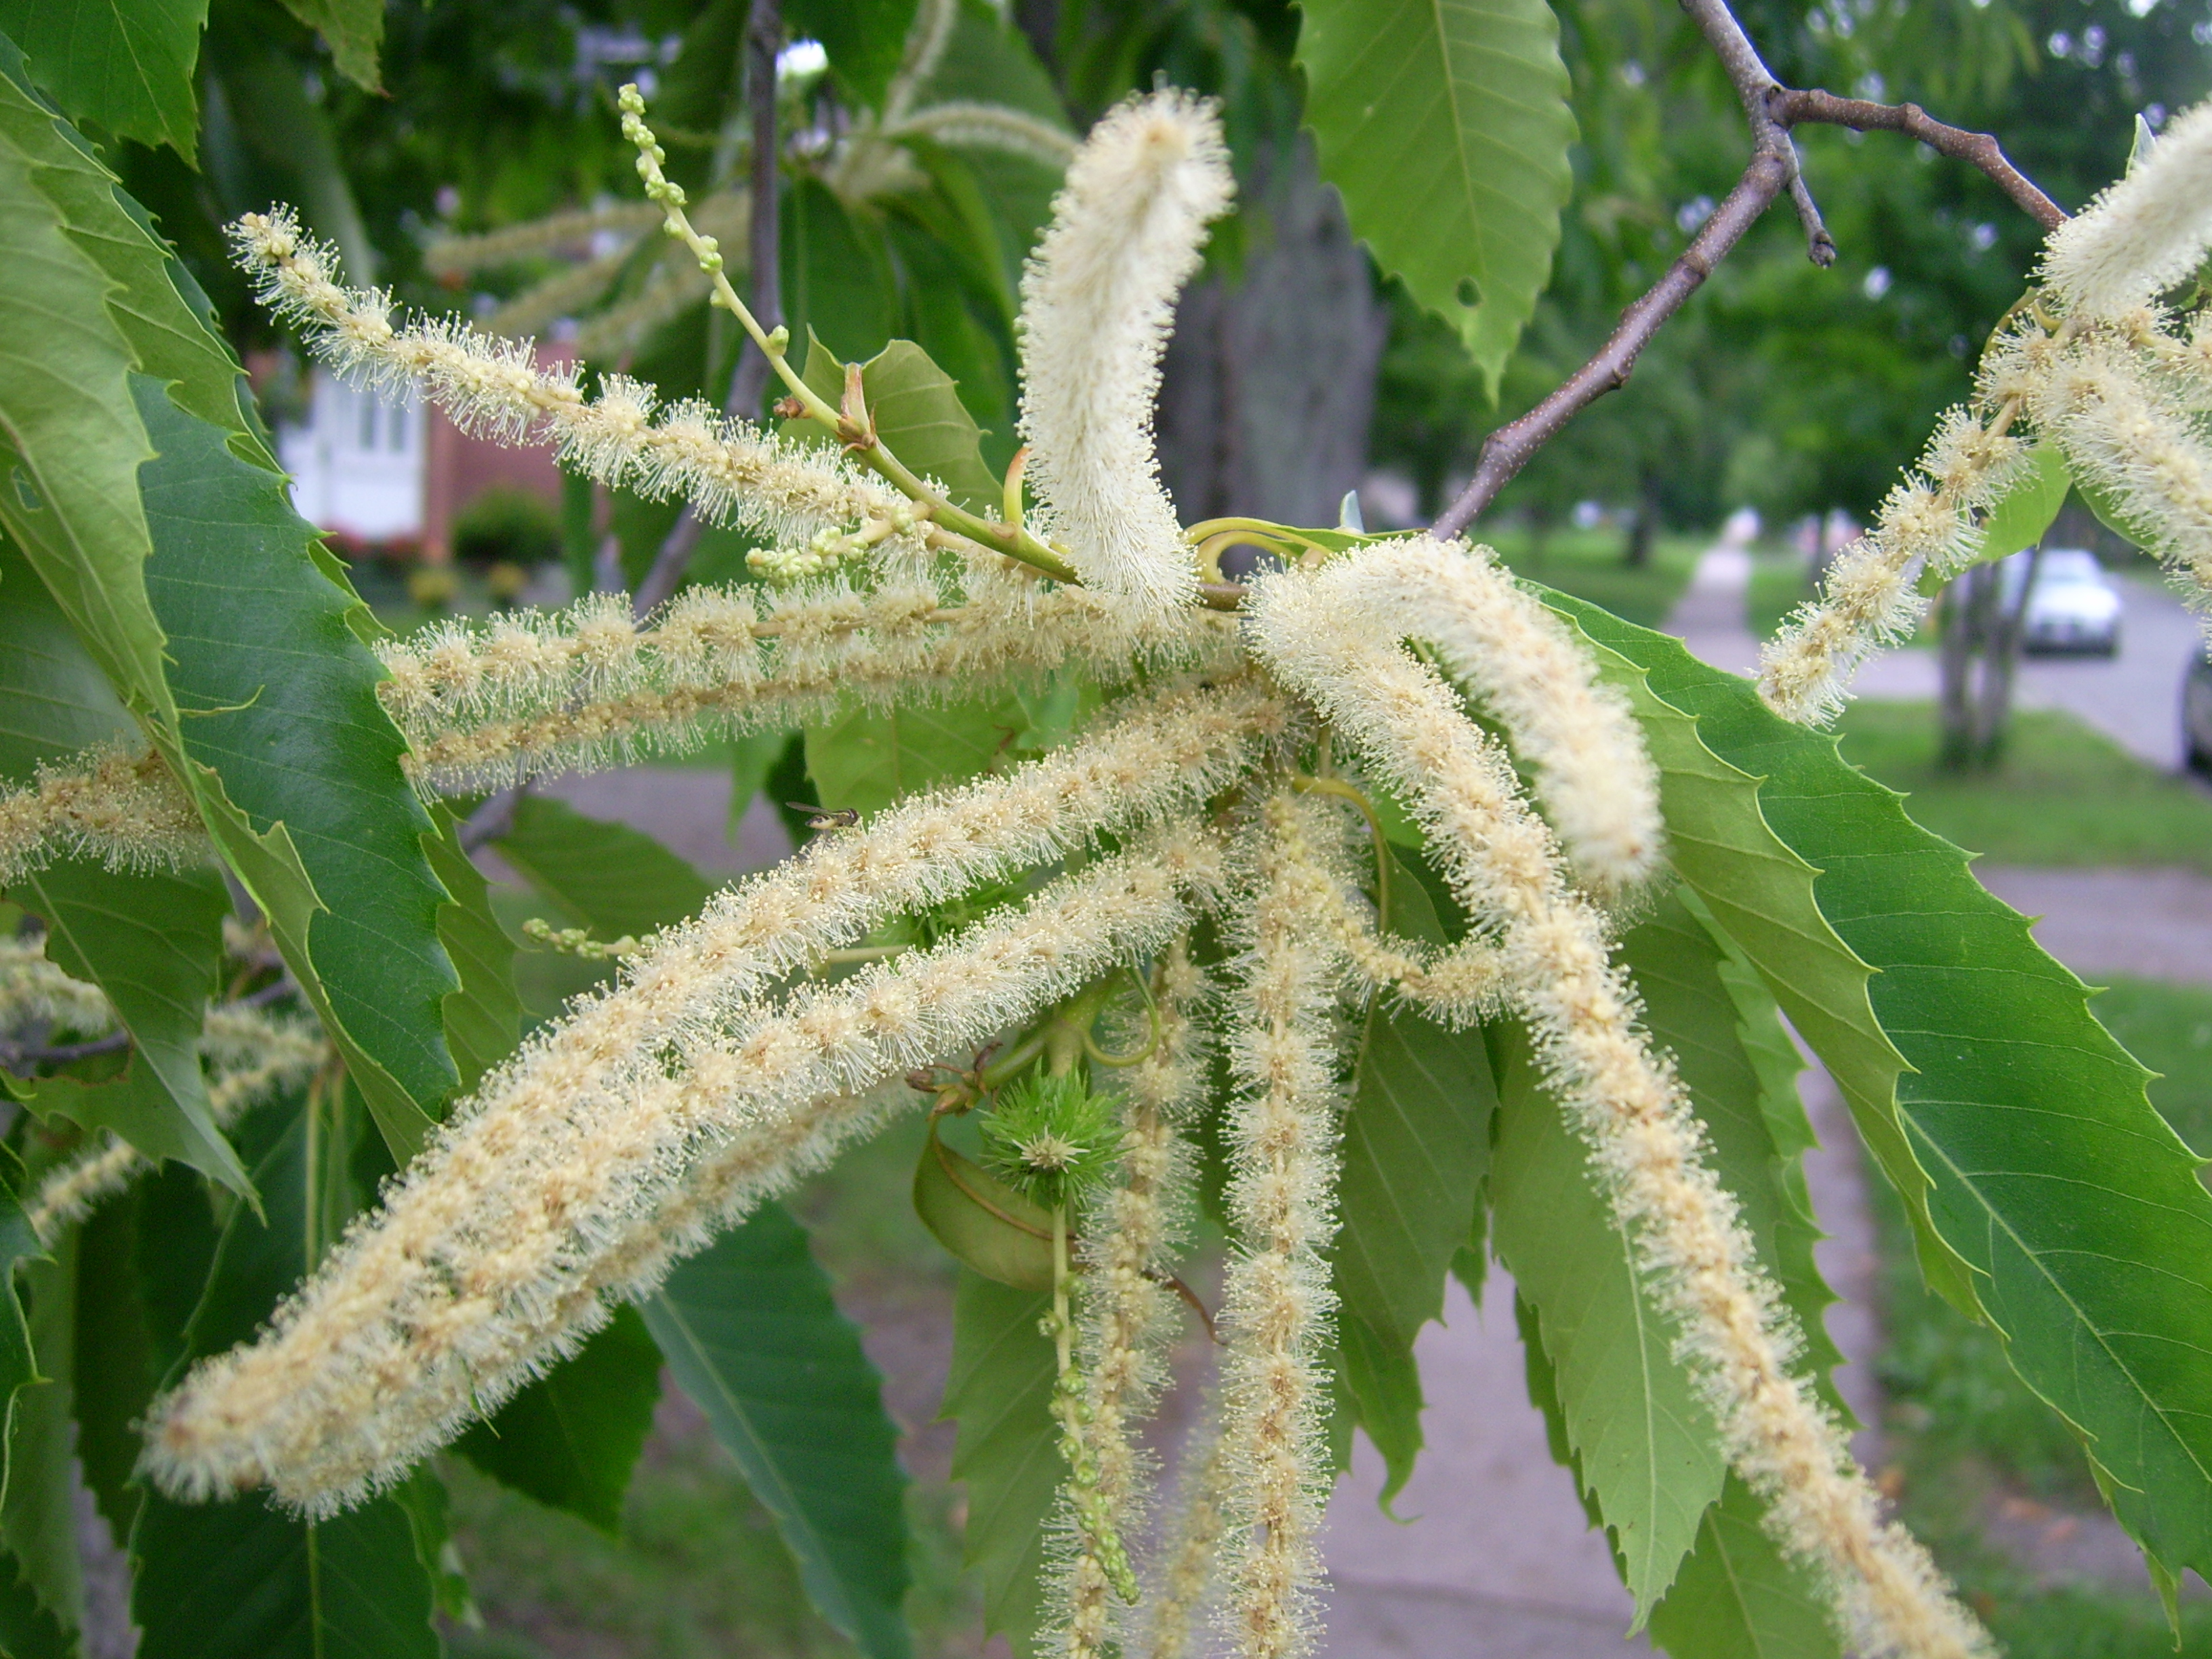
\includegraphics[width=0.5\linewidth]{castflower} 

}

\caption{*Castanea dentata* leaves (left), flowers on catkins (right).}\label{fig:cast}
\end{figure}

\emph{Castenea dantata} was once prolific across the Eastern U.S., but has faced rapid decline of it's historic range following introduction of a pathogenic fungus in New York City in 1904. The chestnut blight, introduced by imported Chinese chestnuts (\emph{Castanea mollissima}), prevents American chestnuts from reaching maturity. Nowadays, trees that resprout from stumps can grow up to 20 feet tall and produce some nuts before succumbing to the blight. Work by the American Chestnut Society is being done to produce blight resistant trees by hybridizing American chestnut with Chinese chestnut. (ACF 2016)

Healthy American chestnuts can grow to be 50-75 feet tall and an equal width of foliage. The leaves can grow between 4 and 9 inches long at a width of 1.5 to 3 inches, that are dark green with coarse-toothed margin and bristly tips. In fall the leaves turn a yellow-gold. Chestnuts flower from June to July, producing yellowish-white flowers on catkins (a cylindrical flower cluster). (NCSU n.d.b)

Further reading; \href{https://acf.org}{American Chestnut Foundation}, \href{https://plants.ces.ncsu.edu/plants/castanea-dentata/}{\emph{Castanea dentata}}

\hypertarget{galax-unceolata}{%
\section{\texorpdfstring{\emph{Galax unceolata}}{Galax unceolata}}\label{galax-unceolata}}

\hypertarget{common-names-wandflower-wandplant-and-beetleweed.}{%
\subsection{Common names; Wandflower, Wandplant, and Beetleweed.}\label{common-names-wandflower-wandplant-and-beetleweed.}}

\begin{figure}

{\centering 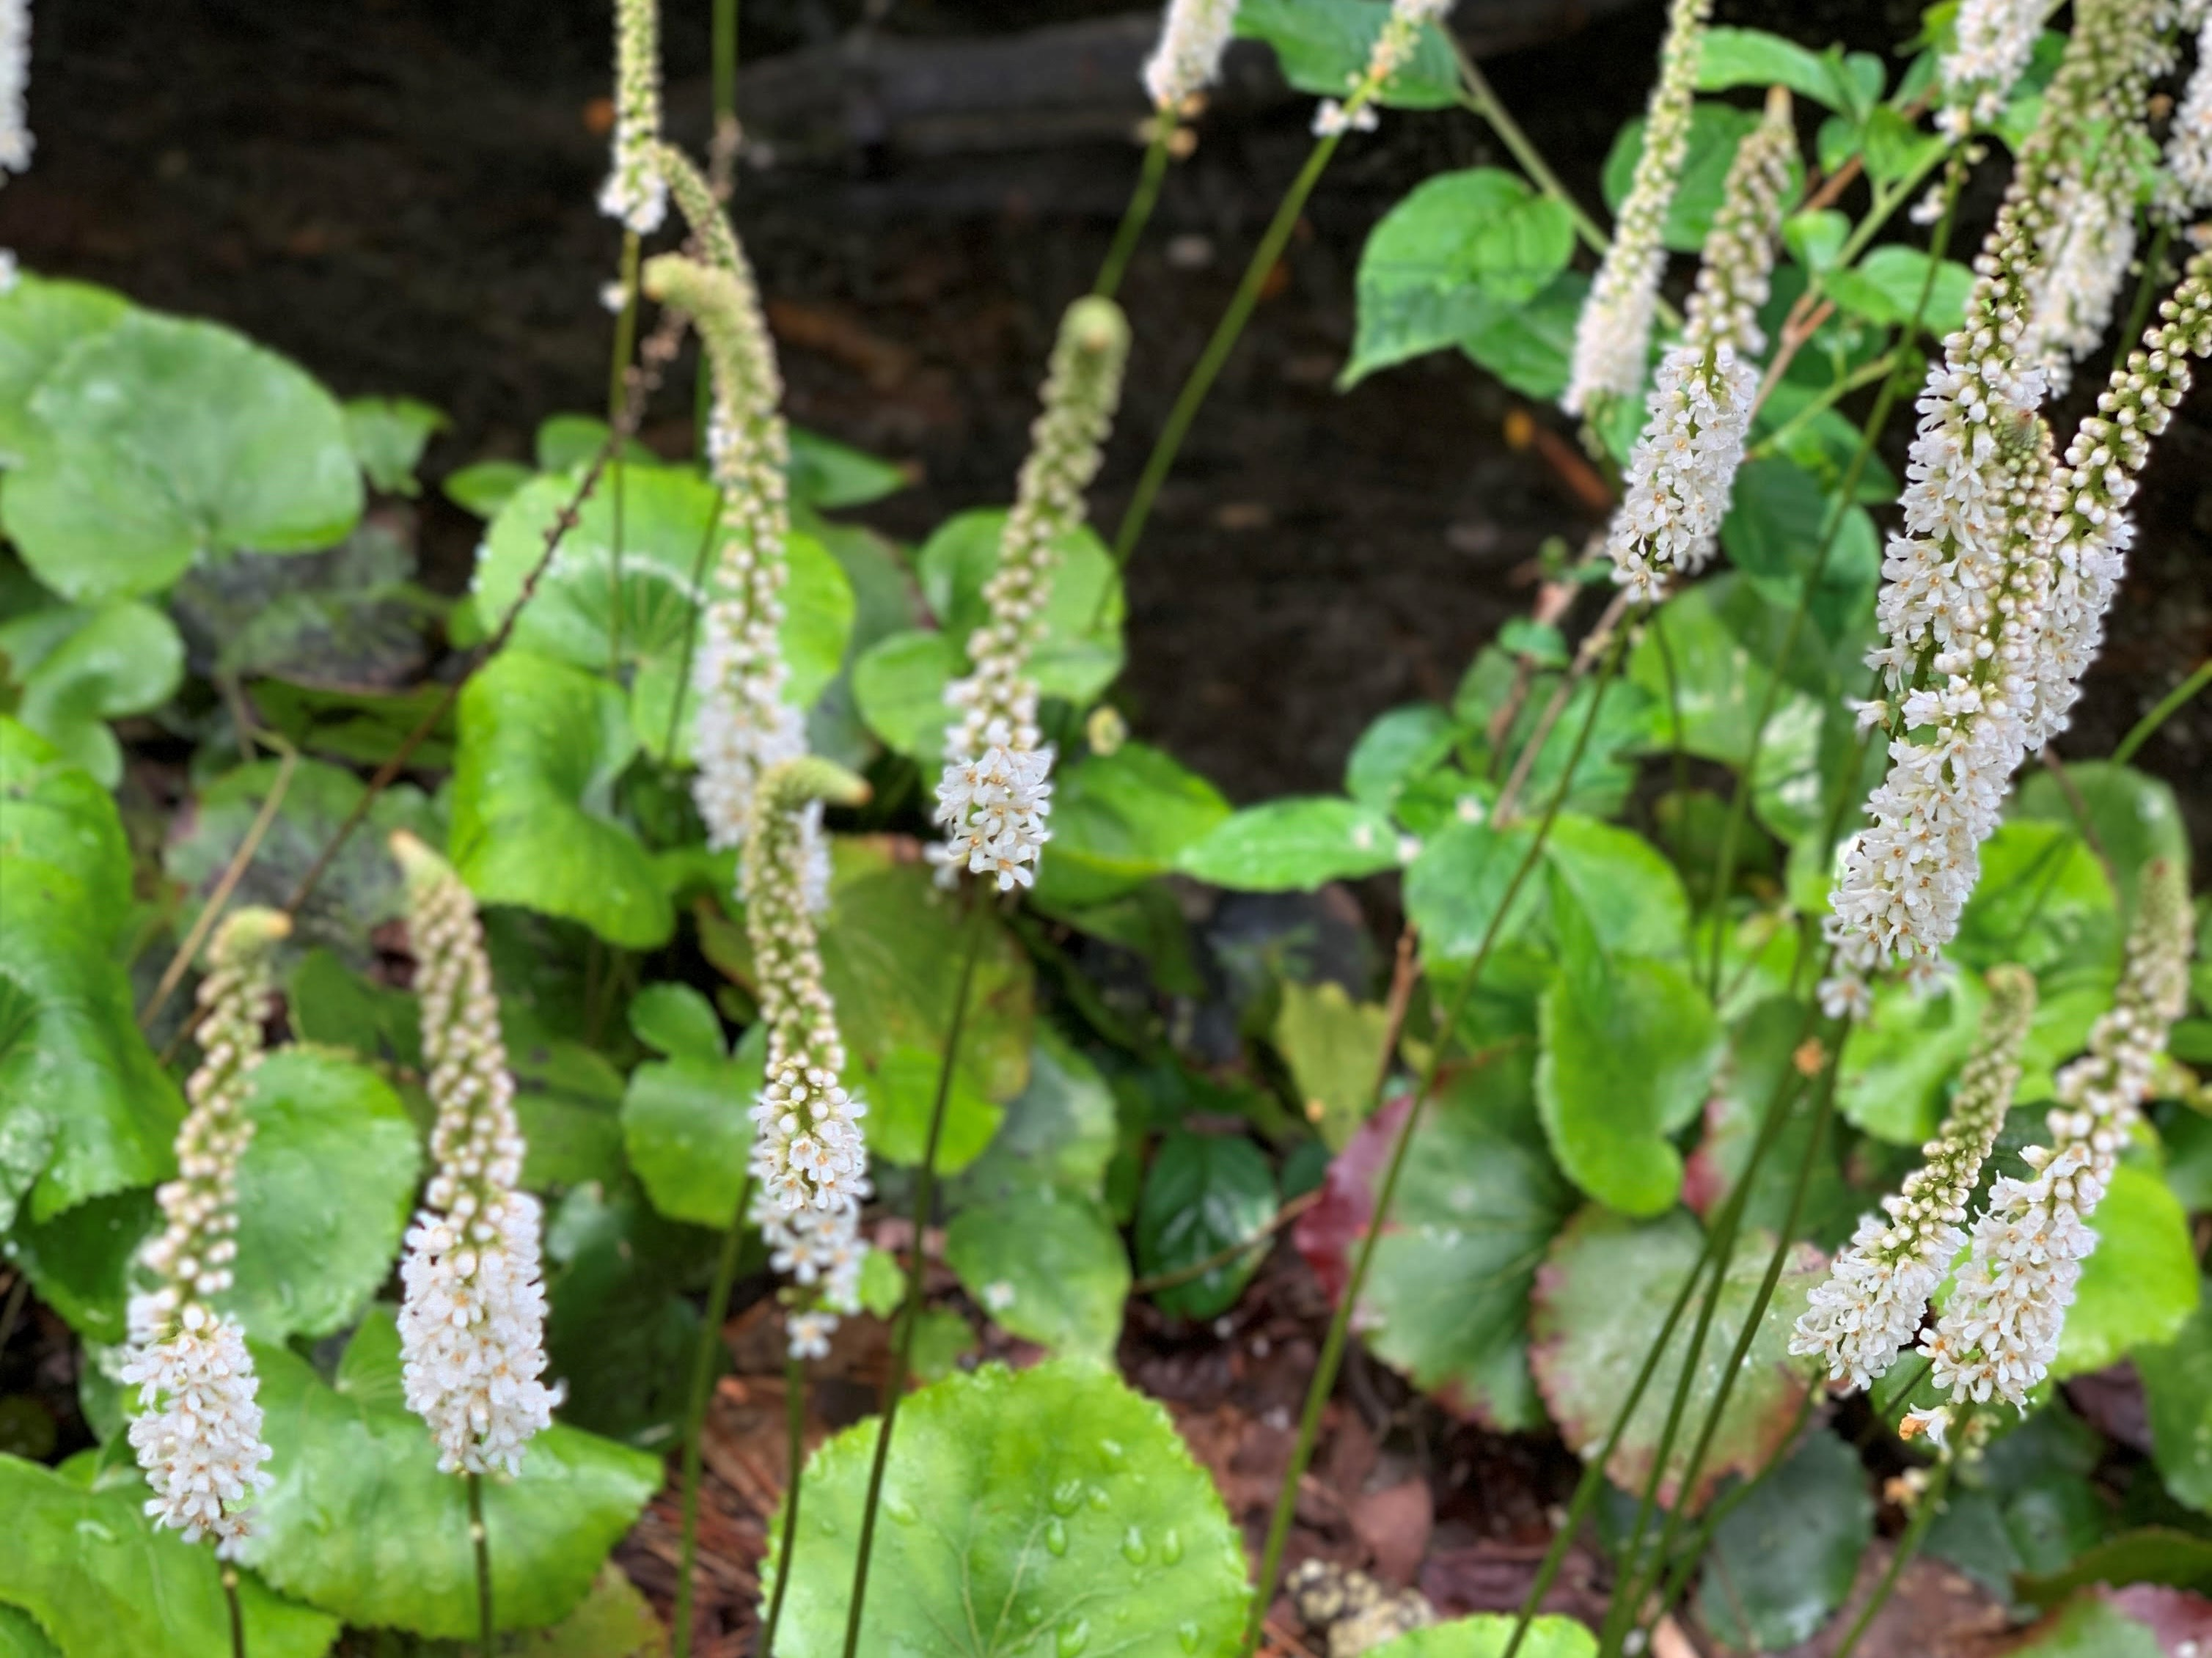
\includegraphics[width=0.5\linewidth]{galax1} 

}

\caption{*Galax unceolata* in bloom.}\label{fig:galax1}
\end{figure}

\emph{Galax unceolata} is an herbaceous perennial plant native to North America, growing mainly in the Appalachian Mountains up to 1500 meters (4921 feet) in elevation. This species is the sole representative of the plant family Diapensiaceae. This plant grows mainly in the understory of shaded forests and is composed of a rosette of leathery cardioid (heart) shaped leaves. The leaves are serrated along the margin and will turn brown during the winter. Galax flowers in late spring to early summer clustered along a single spike-like stem. Each individual flower is composed of five petals and are white in color. The leaves persist throughout the year and are commonly harvested and used as an herbal remedy for cuts and kidney ailments. Although Galax is secure in the Southern Appalachian region, there are concerns about over harvesting in the northern extent of its range. (Predny and Chamberlain 2005)

Further reading; \href{https://www.srs.fs.usda.gov/pubs/gtr/gtr_srs087.pdf}{Galax (\emph{Galax unceolata}): An Annotated Bibliography}

\hypertarget{gaylussacia-spp.}{%
\section{\texorpdfstring{\emph{Gaylussacia spp.}}{Gaylussacia spp.}}\label{gaylussacia-spp.}}

\hypertarget{common-names-huckleberry-and-dangleberry}{%
\subsection{Common names; Huckleberry and Dangleberry}\label{common-names-huckleberry-and-dangleberry}}

\begin{figure}

{\centering 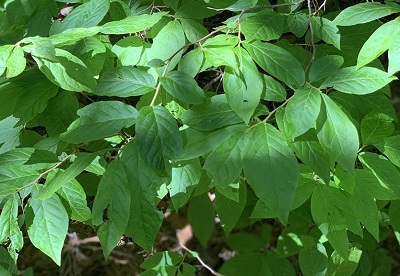
\includegraphics[width=0.5\linewidth]{galuss} 

}

\caption{Foliage of Gaylussacia in a sun fleck.}\label{fig:gayluss}
\end{figure}

\emph{Gaylussacia} is a genus of flowering plants that contains about 50 different species in the Ericaceae family. These deciduous or evergreen shrubs (depending on species) are a common component of oak-heath forests and are native to the Americas. These plant species are used as food by Lepidoptera (butterflies and moths) larvae, including \emph{Coleophora gaylussaciella} which feeds exclusively on these plants. The fruits are edible to humans and are dark purple-black colored berries similar to blueberries (\emph{Vacciunium spp.}). (n.d.a)

Further reading; \href{https://www.fs.fed.us/wildflowers/beauty/mycotrophic/monotropa_hypopitys.shtml}{\emph{Gaylussacia baccata} --- black huckleberry}

\hypertarget{iris-sanguinea}{%
\section{\texorpdfstring{\emph{Iris sanguinea}}{Iris sanguinea}}\label{iris-sanguinea}}

\hypertarget{common-names-japanese-iris-and-siberian-iris}{%
\subsection{Common names; Japanese Iris and Siberian Iris}\label{common-names-japanese-iris-and-siberian-iris}}

\begin{figure}

{\centering 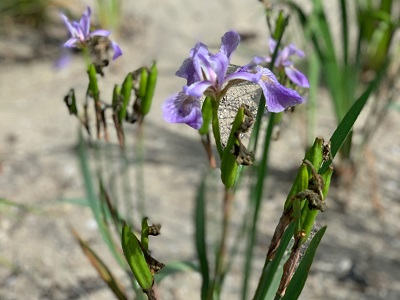
\includegraphics[width=0.5\linewidth]{irissan} 

}

\caption{*Iris sanguinea* in late bloom.}\label{fig:iris}
\end{figure}

\emph{Iris sanguinea} is native to eastern Asia, hence the common names, but have since been naturalized to temperate regions across the globe. Many plants of this genus are poisonous if ingested, especially the roots, as such they are resistant to deer and rabbits. Iris can grow in virtually every hardiness region of the U.S. but particularly enjoys deep meadows, near riparian areas, and on forest edges. The soils for this plant should be well draining, with slight acidity and plenty of organic matter. It prefers full sun but is tolerant of partial shade. It flowers between May and July, producing blue, white, or purple-lavendar showy blooms. The flower goes to seed in July through September following flower blooms. The seeds, themselves, are ellipsoidal capsules with with flat seeds. (NCSU n.d.c, PFAF n.d.)

Further reading; \href{https://plants.ces.ncsu.edu/plants/iris-sanguinea/}{\emph{Iris sanguinea}},
\href{https://pfaf.org/user/Plant.aspx?LatinName=Iris+sanguinea}{Iris sanguinea - Donn. ex Hornem.}

\hypertarget{kalmia-latifolia}{%
\section{\texorpdfstring{\emph{Kalmia latifolia}}{Kalmia latifolia}}\label{kalmia-latifolia}}

\hypertarget{common-names-calico-bush-ivy-bush-laurel-mountain-ivy-mountain-laurel-sheepkill-and-spoonwood}{%
\subsection{Common names; Calico bush, Ivy bush, Laurel, Mountain ivy, Mountain laurel, Sheepkill, and Spoonwood}\label{common-names-calico-bush-ivy-bush-laurel-mountain-ivy-mountain-laurel-sheepkill-and-spoonwood}}

\begin{figure}

{\centering 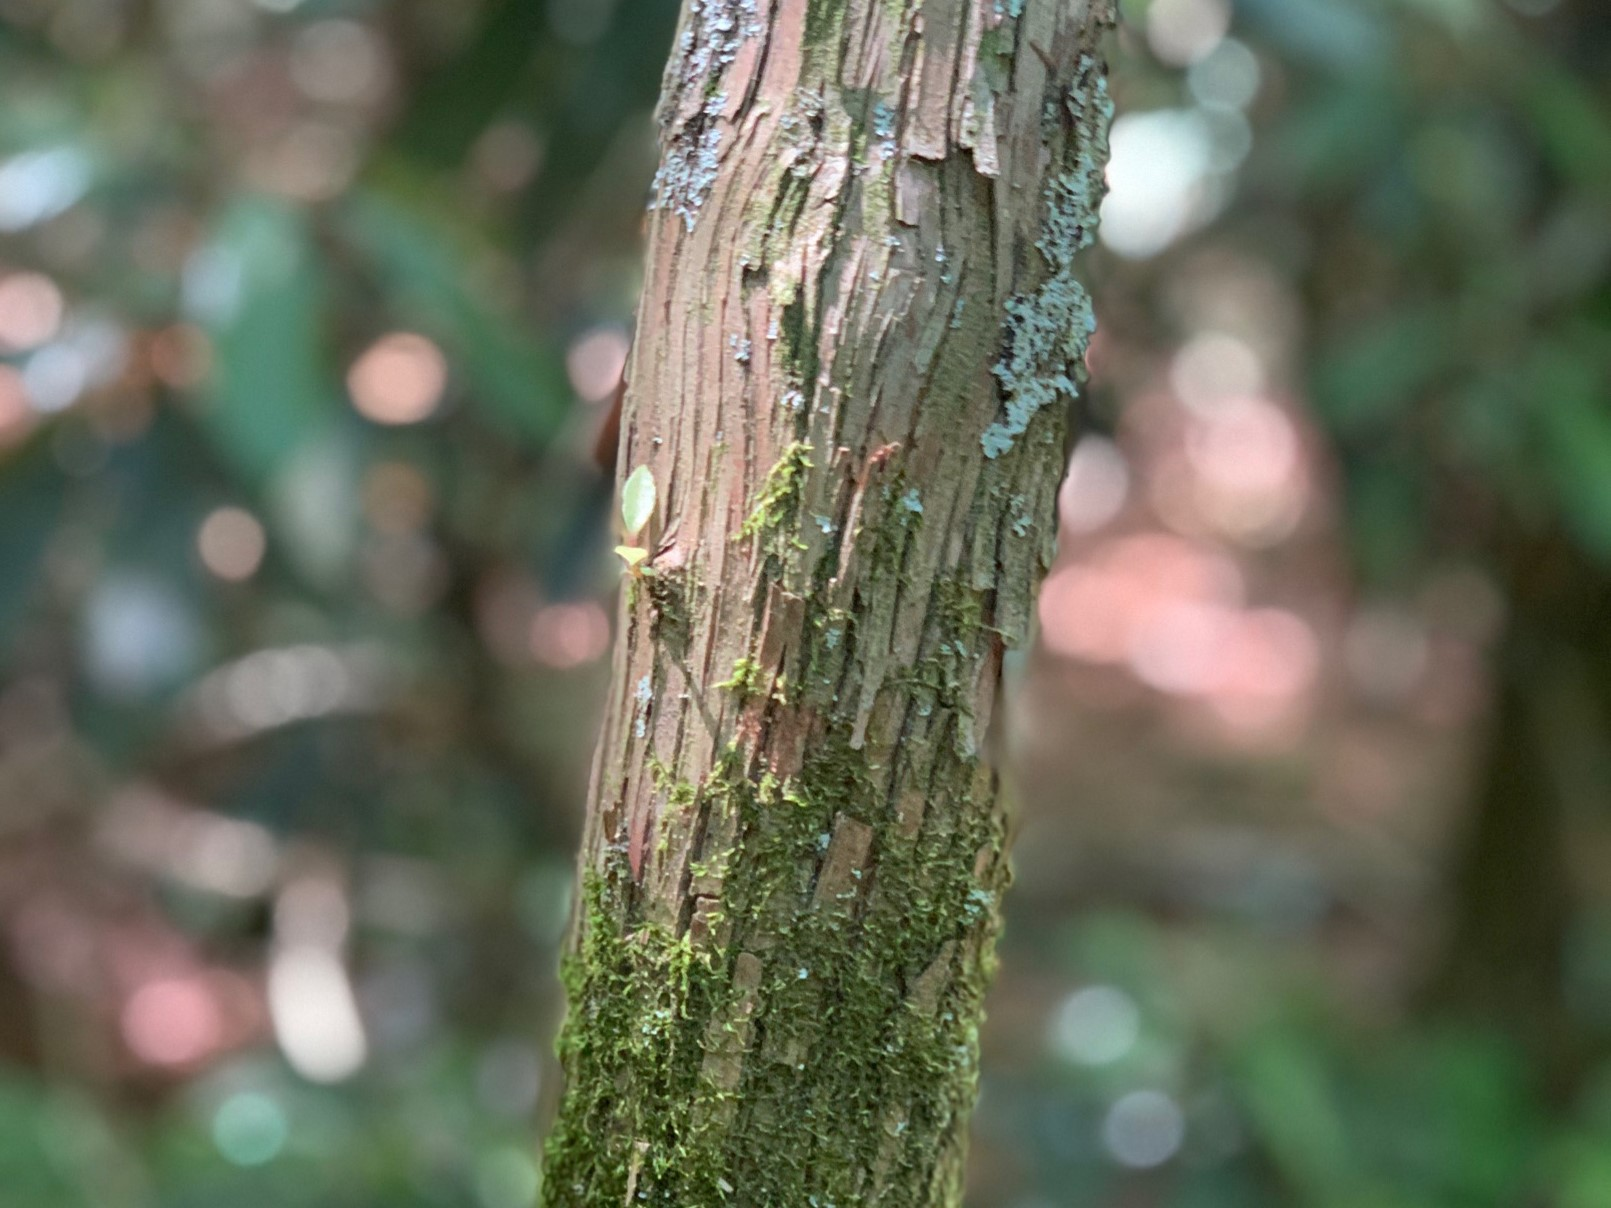
\includegraphics[width=0.5\linewidth]{kalmia1} 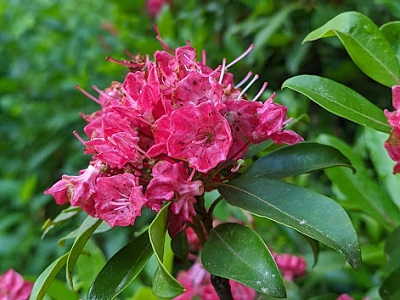
\includegraphics[width=0.5\linewidth]{kalmlat} 

}

\caption{*Kalmia latifolia* bark (top left), pink flowers in bloom (top right).}\label{fig:kalmia}
\end{figure}

\emph{Kalmia latifolia} is a broadleaf evergreen shrub that often branches into a thicket and sometimes as a small tree with a crooked trunk. Laurel flowers in late April to July for several weeks in a range of colors from pink or purple/lavender to white. Each flower is cup-shaped with 4-5 petals and begin fruiting in Fall. Fruits are capsules that are brown or copper in color and present from September to October. Laurel is highly poisonous affecting skeletal muscle and cardiac muscle function, as well as nerve function. Laurel is commonly mistaken for \emph{Rhododendron spp.} due to similar leaf structure, laurel has smaller leaves and rhododendron have larger leaves. Likewise, as laurel ages the bark begins to peel off in long strips. The two are otherwise similar in growth requirements, i.e.~full sun or partial shade, acidic soils with good drainage and high organic matter. (TWC 2017a, Figart 2021, NCSU n.d.d)

Further reading; \href{https://www.wildflower.org/plants/result.php?id_plant=KALA}{\emph{Kalmia latifolia}}, \href{https://www.smokiesinformation.org/news/wildflowers-101-mountain-laurel-and-rhododendron.html\#:~:text=The\%20laurel\%20has\%20the\%20smaller,leaves\%20droop\%20and\%20curl\%20back.}{WILDFLOWERS 101: MOUNTAIN LAUREL AND RHODODENDRON}, \href{https://plants.ces.ncsu.edu/plants/kalmia-latifolia/}{\emph{Kalmia latifolia}}

\hypertarget{laetiporous-sulphureus}{%
\section{\texorpdfstring{\emph{Laetiporous sulphureus}}{Laetiporous sulphureus}}\label{laetiporous-sulphureus}}

\hypertarget{common-names-chicken-of-the-woods-chicken-fungus-chicken-mushroom-crab-of-the-woods-sulphur-polypore-and-sulphur-shelf}{%
\subsection{Common names; Chicken-of-the-woods, Chicken fungus, Chicken mushroom, Crab-of-the-woods, Sulphur polypore, and Sulphur shelf}\label{common-names-chicken-of-the-woods-chicken-fungus-chicken-mushroom-crab-of-the-woods-sulphur-polypore-and-sulphur-shelf}}

\begin{figure}

{\centering 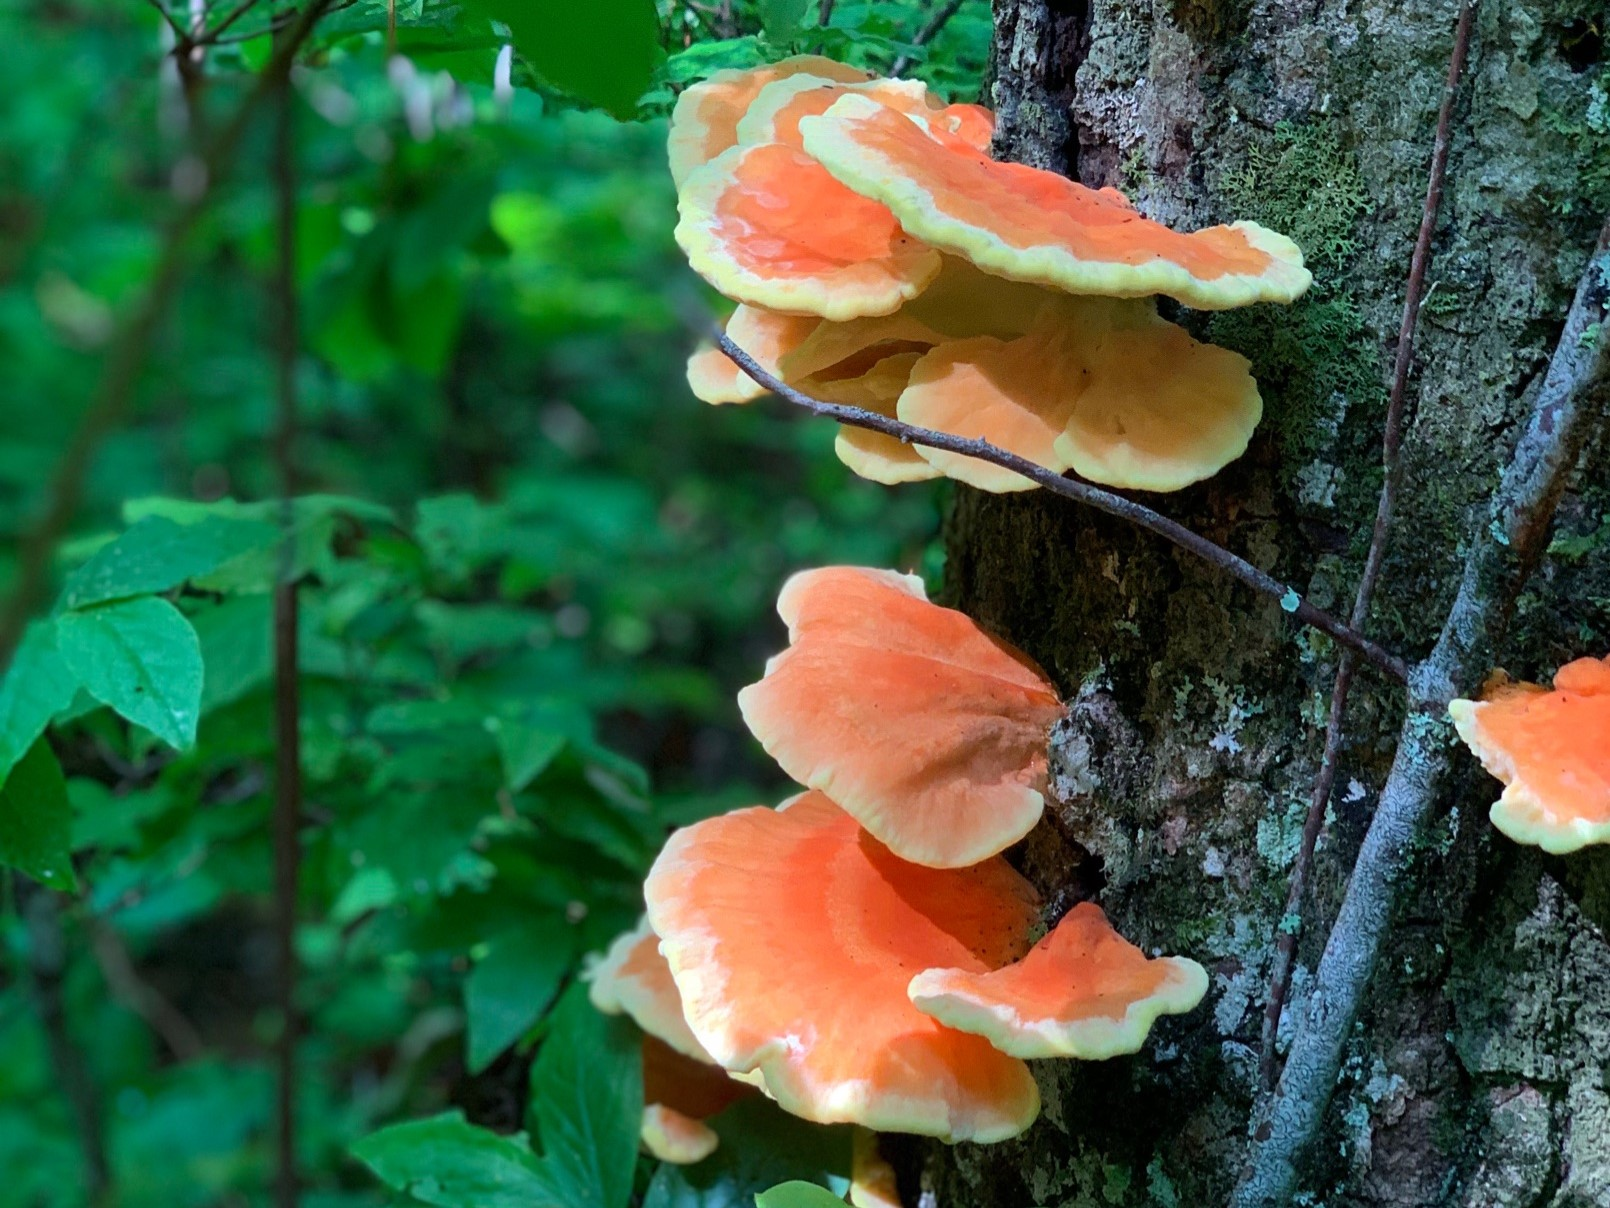
\includegraphics[width=0.5\linewidth]{chicken} 

}

\caption{*Laetiporous sulphureus* ripe for harvesting.}\label{fig:chicken}
\end{figure}

\emph{Laetiporous sulphureus} is an edible polypore that is described as having the taste and texture of chicken meat. This fungus grows in shelf-like fashion on the bark of dead trees most commonly; beech, oak, and chestnut, occasionally on cherry or other hardwoods. When the fungus fruits it displays on the bark as vibrant orange or sulphur-yellow with a pale yellow or white underside. Individual shelves can grow 10 to 40 cm in width and vary in thickness from 3 to 12 cm. The flesh will retain its coloration when moist and ripe but will dry out to a paler coloration before decaying into a black mush. Likewise, the flesh will feel tender when young and become tough with age. Chicken-of-the-woods can sometimes be mistaken for the paler Giant Polypore (\emph{Meripilus giganteus}) which can be distinguished by bruising the pores - if they turn black, it's Giant Polypore. This lookalike is also edible but tastes like cardboard and can cause an upset stomach in some individuals. (Kuo 2017, Mrs. Mushroom 2022, O'Reilly and Parker n.d.)

Further reading; \href{https://www.first-nature.com/fungi/laetiporus-sulphureus.php}{Laetiporus sulphureus (Bull.) Murrill - Chicken-of-the-Woods}, \href{https://www.mushroom-appreciation.com/chicken-of-the-woods.html}{Chasing the Chicken of the Woods (Facts, Identification, and Recipes)},
\href{https://www.mushroomexpert.com/laetiporus_sulphureus.html}{Laetiporus sulphureus}

\hypertarget{liriodendron-tulipifera}{%
\section{\texorpdfstring{\emph{Liriodendron tulipifera}}{Liriodendron tulipifera}}\label{liriodendron-tulipifera}}

\hypertarget{common-names-blue-poplar-tulip-poplar-tulip-tree-yellow-poplar-yellow-wood}{%
\subsection{Common names; Blue-poplar, Tulip-poplar, Tulip tree, Yellow-poplar, Yellow wood}\label{common-names-blue-poplar-tulip-poplar-tulip-tree-yellow-poplar-yellow-wood}}

\begin{figure}

{\centering 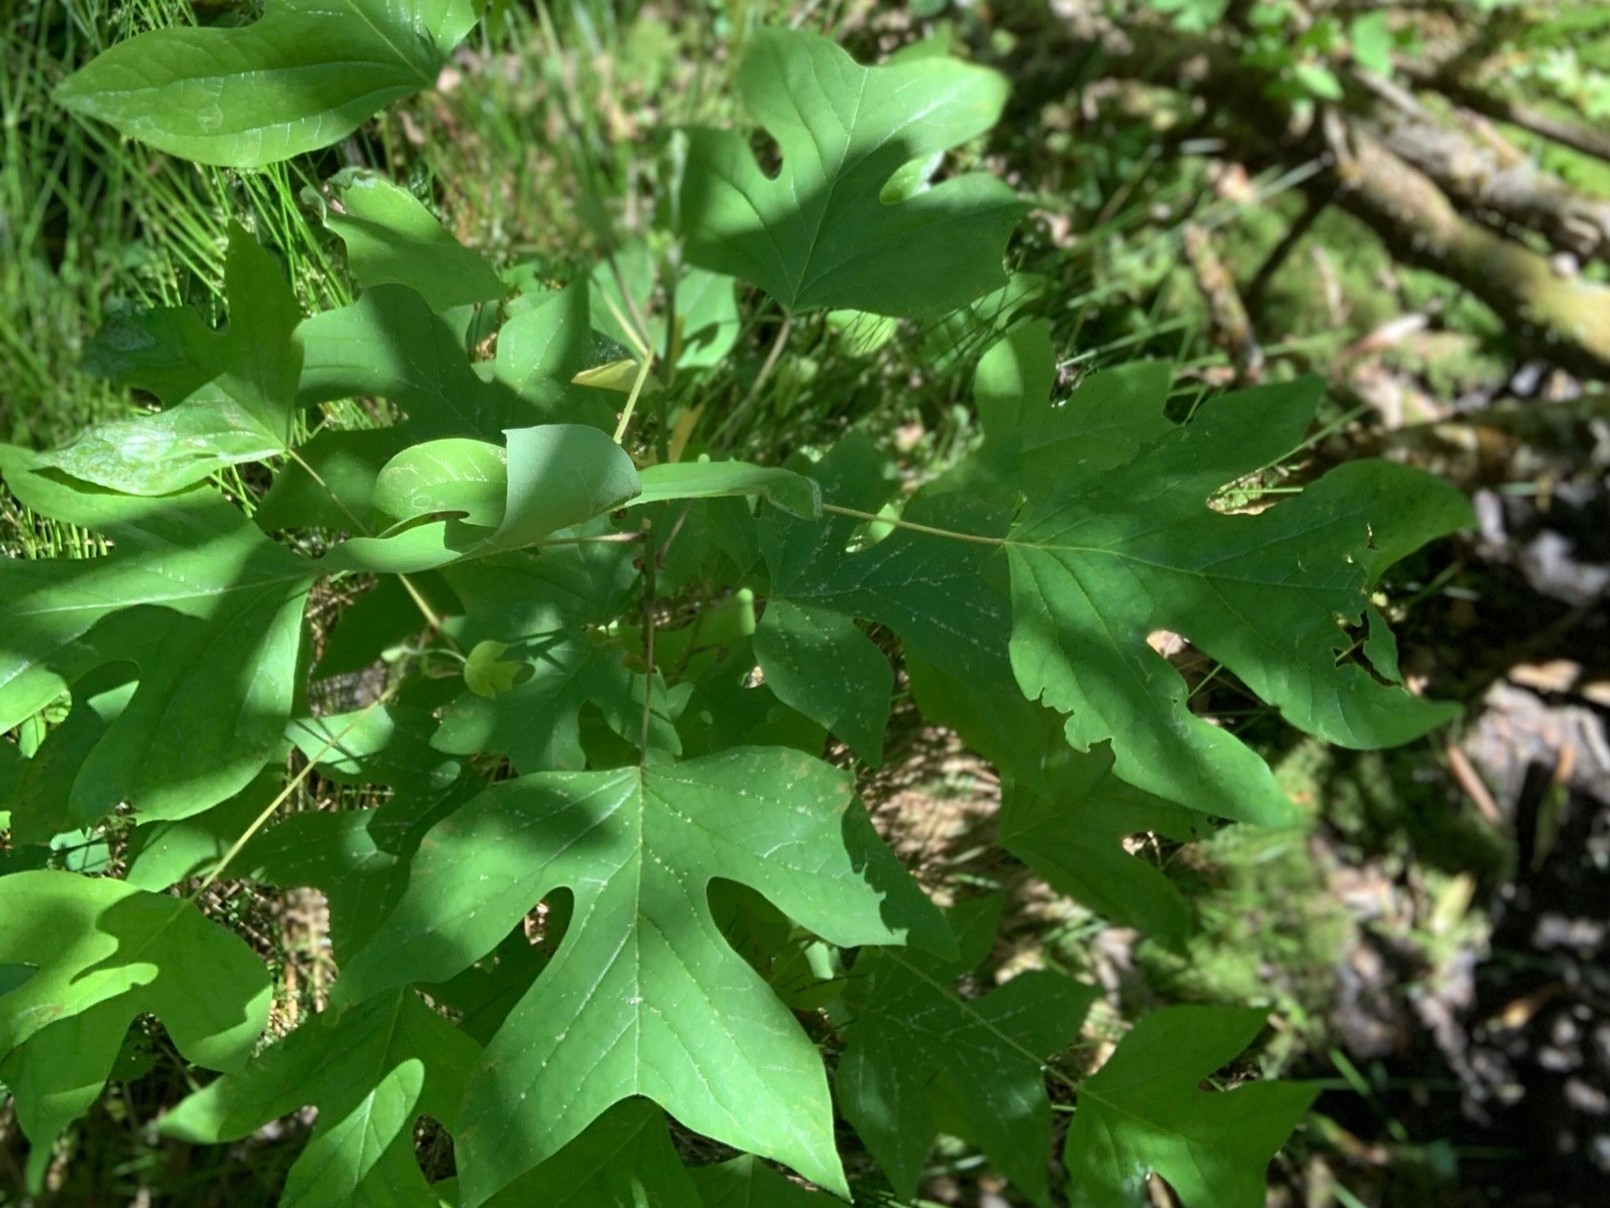
\includegraphics[width=0.5\linewidth]{tulip} 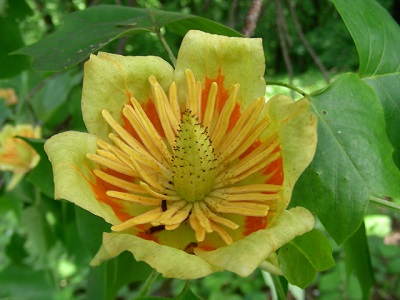
\includegraphics[width=0.5\linewidth]{tulipflower} 

}

\caption{*Liriodendron tulipifera* leaves in a sun fleck (left), floral bloom (right).}\label{fig:tulippop}
\end{figure}

\emph{Liriodendron tulipifera} is a deciduous pioneer tree species, meaning it is one of the first species to fill a disturbance gap in a forest stand. These trees are fast-growing without the constraint of weak wood, making it a valuable timber species. As such the wood from this tree is often used for furniture, as veneer, in boats, as paper pulp, and general lumber. In medicinal terms the inner bark was used by the First Nations as a worming medicine, an anti-arthritic, a cough syrup, and as a remedy for cholera. For wildlife this tree is a favorite of nesting birds, the flowers attract hummingbirds, and is a larval host for the Eastern Tiger Swallowtail butterfly (\emph{Papilio glaucus}). Flowers will bloom between April and June, producing fragrant and edible cup-shaped flowers each with 6 petals. The flowers can present as gold/yellow, green, or orange in coloration. On larger trees they can be hard to spot as they bloom after the leaves are fully developed, only noticeable once they begin to fall. (TWC 2021, NCSU n.d.e)

Further reading; \href{https://plants.ces.ncsu.edu/plants/liriodendron-tulipifera/}{Liriodendron tulipifera}, \href{https://www.wildflower.org/plants/result.php?id_plant=LITU}{Liriodendron tulipifera}

\hypertarget{monotropa-uniflora}{%
\section{\texorpdfstring{\emph{Monotropa uniflora}}{Monotropa uniflora}}\label{monotropa-uniflora}}

\hypertarget{common-names-indian-pipe-and-ghost-plant}{%
\subsection{Common names; Indian Pipe and Ghost Plant}\label{common-names-indian-pipe-and-ghost-plant}}

\begin{figure}

{\centering 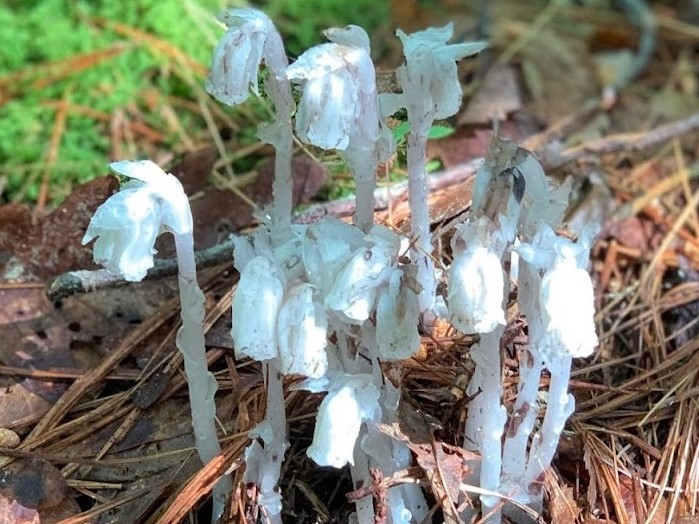
\includegraphics[width=0.5\linewidth]{M uniflora} 

}

\caption{*Monotropa uniflora* flowers.}\label{fig:uniflora}
\end{figure}

\emph{Monotropa uniflora} is a perennial wildflower that grows to height between 10 and 30 cm. \emph{M uniflora} blooms in early summer through early autumn in mature, moist, shaded forests. This plant is entirely translucent white while sometimes appearing in a pale pinkish-hue. This is because the plant is parasitic in nature and obtains its nutrients from photosynthetic trees (commonly Beech; \emph{Fagus sp.}) connected via fungal mycorrhizal networks. The leaves that arise directly from the peduncle (flower stalk) are scale-like and can be flecked black. As the name suggests - uniflora - this plant has single-flowers that emerge as pendants (pointed downward). Once the flower matures it erects perpendicular to the stalk. The fruits are capsules with seeds that release through slits along the length of the capsule. The flowers can persist following seed dispersal however the flesh may become desiccated and look brown or black. (USFS n.d.)

Further reading; \href{https://www.fs.fed.us/wildflowers/beauty/mycotrophic/monotropa_uniflora.shtml}{\emph{Monotropa uniflora} - Ghost Plant, Indian Pipe}

\hypertarget{onoclea-struthiopteris}{%
\section{\texorpdfstring{\emph{Onoclea struthiopteris}}{Onoclea struthiopteris}}\label{onoclea-struthiopteris}}

\hypertarget{common-names-fiddlehead-fern-ostrich-feather-fern-ostrich-fern-and-shuttlecock-fern}{%
\subsection{Common names; Fiddlehead fern, Ostrich-feather fern, Ostrich fern, and Shuttlecock fern}\label{common-names-fiddlehead-fern-ostrich-feather-fern-ostrich-fern-and-shuttlecock-fern}}

\begin{figure}

{\centering 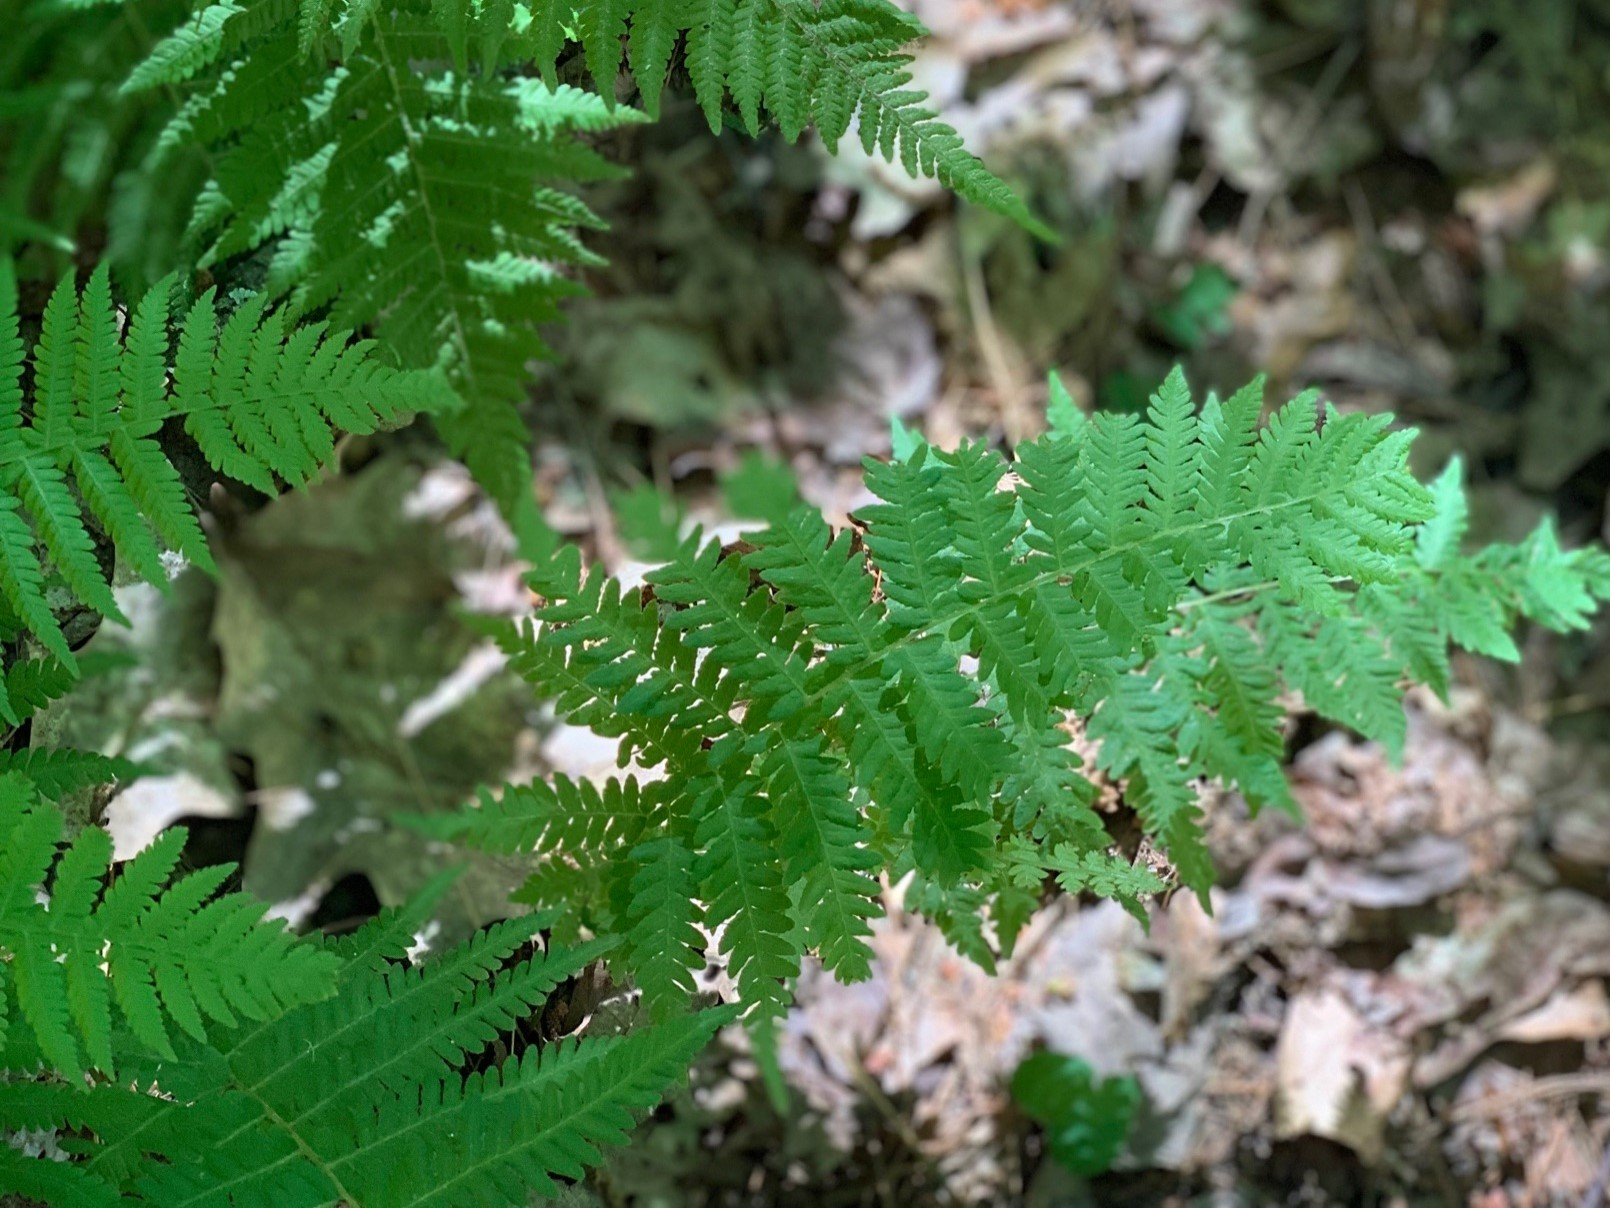
\includegraphics[width=0.5\linewidth]{fern} 

}

\caption{*Onoclea struthiopteris* fronds.}\label{fig:shutfern}
\end{figure}

\emph{Onoclea struthiopteris} is a perennial and deciduous fern often found in moist areas, in thickets, and in the understory of trees. Ostrich fern prefers partial to full shade, but will tolerate full sun with moist soils and cool temperatures. This plant is resistant to browsing by deer but the emerging fiddleheads are otherwise edible. It has the potential to prevent erosion due to its rhizomatous colonization of the topsoil. Caution should be taken if planting in small spaces as it can spread aggressively. (TWC 2017b, NCSU n.d.f)

Futher reading; \href{https://www.wildflower.org/plants/result.php?id_plant=MAST}{\emph{Matteuccia struthiopteris}} (although a different latin name, this is synonymous with \emph{O. struthiopteris}),
\href{https://plants.ces.ncsu.edu/plants/onoclea-struthiopteris/}{\emph{Onoclea struthiopteris}}

\hypertarget{patera-clarki-nantahala}{%
\section{\texorpdfstring{\emph{Patera clarki nantahala}}{Patera clarki nantahala}}\label{patera-clarki-nantahala}}

\hypertarget{common-names-noonday-globe}{%
\subsection{Common names; Noonday globe}\label{common-names-noonday-globe}}

\begin{figure}

{\centering 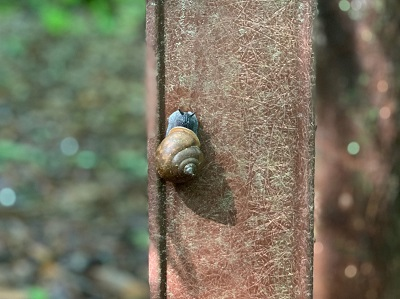
\includegraphics[width=0.5\linewidth]{snail} 

}

\caption{*Patera clarki nantahala* ascending a trail post.}\label{fig:snaily}
\end{figure}

\emph{Patera clarki} is a land snail from the Polygyridae family that is native to the southeastern U.S., specifically; Georgia, North and South Carolina, and Tennessee. There is little information regarding the diet, life cycle, or interspecific interactions due to its rarity and limited distribution. In July of 1978, US Fish and Wildlife placed the noonday globe snail on the Federal Endangered and Threatened Species List, with a fine of as much as \$50,000 and one year in jail for taking one of these snails. (Wikipedia 2021)

\hypertarget{pinus-echinata}{%
\section{\texorpdfstring{\emph{Pinus echinata}}{Pinus echinata}}\label{pinus-echinata}}

\hypertarget{common-names-arkansas-soft-pine-old-field-pine-shortleaf-pine-shortleaf-yellow-pine-shortstraw-pine-southern-yellow-pine-and-yellow-pine}{%
\subsection{Common names; Arkansas soft pine, Old field pine, Shortleaf pine, Shortleaf yellow pine, Shortstraw pine, Southern yellow pine, and Yellow pine}\label{common-names-arkansas-soft-pine-old-field-pine-shortleaf-pine-shortleaf-yellow-pine-shortstraw-pine-southern-yellow-pine-and-yellow-pine}}

\begin{figure}

{\centering 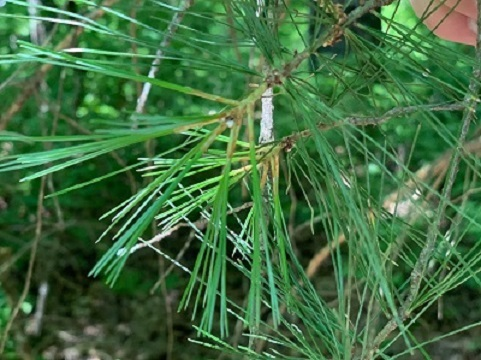
\includegraphics[width=0.5\linewidth]{shortpine} 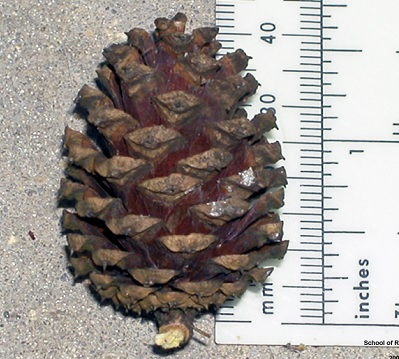
\includegraphics[width=0.5\linewidth]{pinecfe} 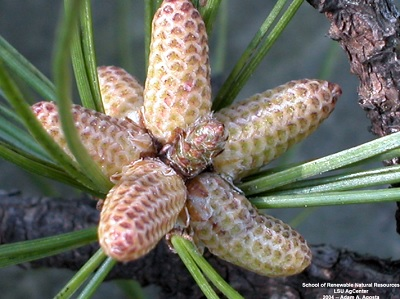
\includegraphics[width=0.5\linewidth]{pinecma} 

}

\caption{Close-up of Short pine needles (top left), female seed cone (top right), male pollen cone (bottom). Cone photos courtesy of LSU School of Renewable Natural Resources [@peccone].}\label{fig:shpine}
\end{figure}

\emph{Pinus echinata} is an evergreen conifer that is native to the southeastern U.S. and is considered one of the hardiest and most adaptable of the southern pines. The limbs will branch out forming a pyramidal crown (wide base to a fine pointed apex) that broadens with age. This tree can grow up to 100 feet tall, with fascicles of 2 or 3 needles between 3 and 5 inches in length. Male trees will produce pale purple cones, while female trees will produce pale pink cones. This pine will grow best in full sun, in well-draining, average wetness, and sandy loam soils. It is also an important timber tree in its more southern range, providing wood for general lumbar, plywood, paper pulp, and turpentine. (n.d.b, NCSU n.d.g)

Further reading; \href{https://www.gardenia.net/plant/pinus-echinata}{\emph{Pinus echinata} (Shortleaf Pine)}, \href{https://plants.ces.ncsu.edu/plants/pinus-echinata/}{\emph{Pinus echinata}}

\hypertarget{pinus-rigida}{%
\section{\texorpdfstring{\emph{Pinus rigida}}{Pinus rigida}}\label{pinus-rigida}}

\hypertarget{common-names-pitch-pine}{%
\subsection{Common names; Pitch pine}\label{common-names-pitch-pine}}

\begin{figure}

{\centering 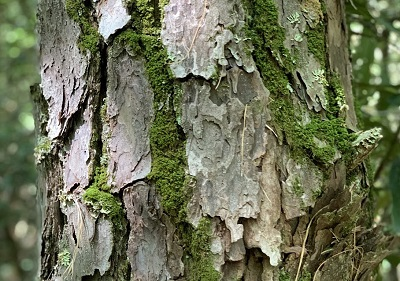
\includegraphics[width=0.5\linewidth]{p rigida bark} 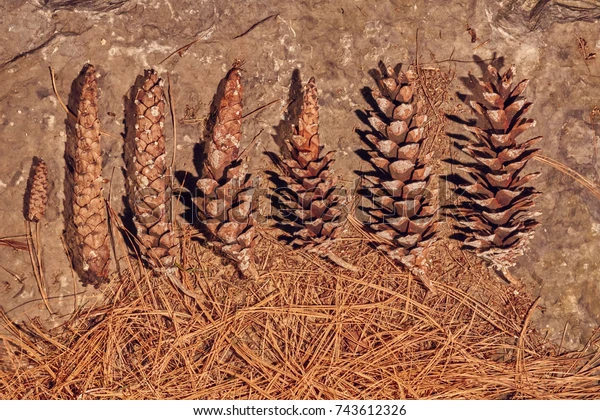
\includegraphics[width=0.5\linewidth]{pitch pine cones} 

}

\caption{*Pinus rigida* bark (Left). Cone life stages (Right), photo courtesy of C. N. Elliot.}\label{fig:rigida}
\end{figure}

\emph{Pinus rigida} is mainly found in the southern areas of the northeastern United States. These trees are found in environments other species may find unfavorable (i.e.~acidic, sandy, and low nutrient soils). The needles of this tree come in fascicles of three, grow to a length of 2 1/4 to 5 inches, and are often slightly twisted. The cones of this tree are serotinous, meaning, they need to be exposed to an internal temperature of 212°F before opening to release seeds. The thick bark provides an adaptation against fire by insulating the sensitive cambium layer from heat and can survive external temperatures as high as 790°F. It also has a remarkable regenerative ability, should it be damaged by cuts or fire, it can resprout using epicormic shoots (growing from the bark). The trunks of pitch pine are usually straight and covered in large, thick, irregular plates of bark. Pitch pine is a pioneer species in abandoned agricultural or pasture land and is replaced by hardwoods, spruce, or other pines in the absence of disturbance. (Gucker 2007)

Further reading; \href{https://www.fs.fed.us/database/feis/plants/tree/pinrig/all.html\#Cone\%20survival\%20and\%20seedling\%20establishment:}{\emph{Pinus rigida}}

\hypertarget{quercus-robur}{%
\section{\texorpdfstring{\emph{Quercus robur}}{Quercus robur}}\label{quercus-robur}}

\hypertarget{common-names-english-oak-oak-and-truffle-oak}{%
\subsection{Common names; English Oak, Oak, and Truffle Oak}\label{common-names-english-oak-oak-and-truffle-oak}}

\begin{figure}

{\centering 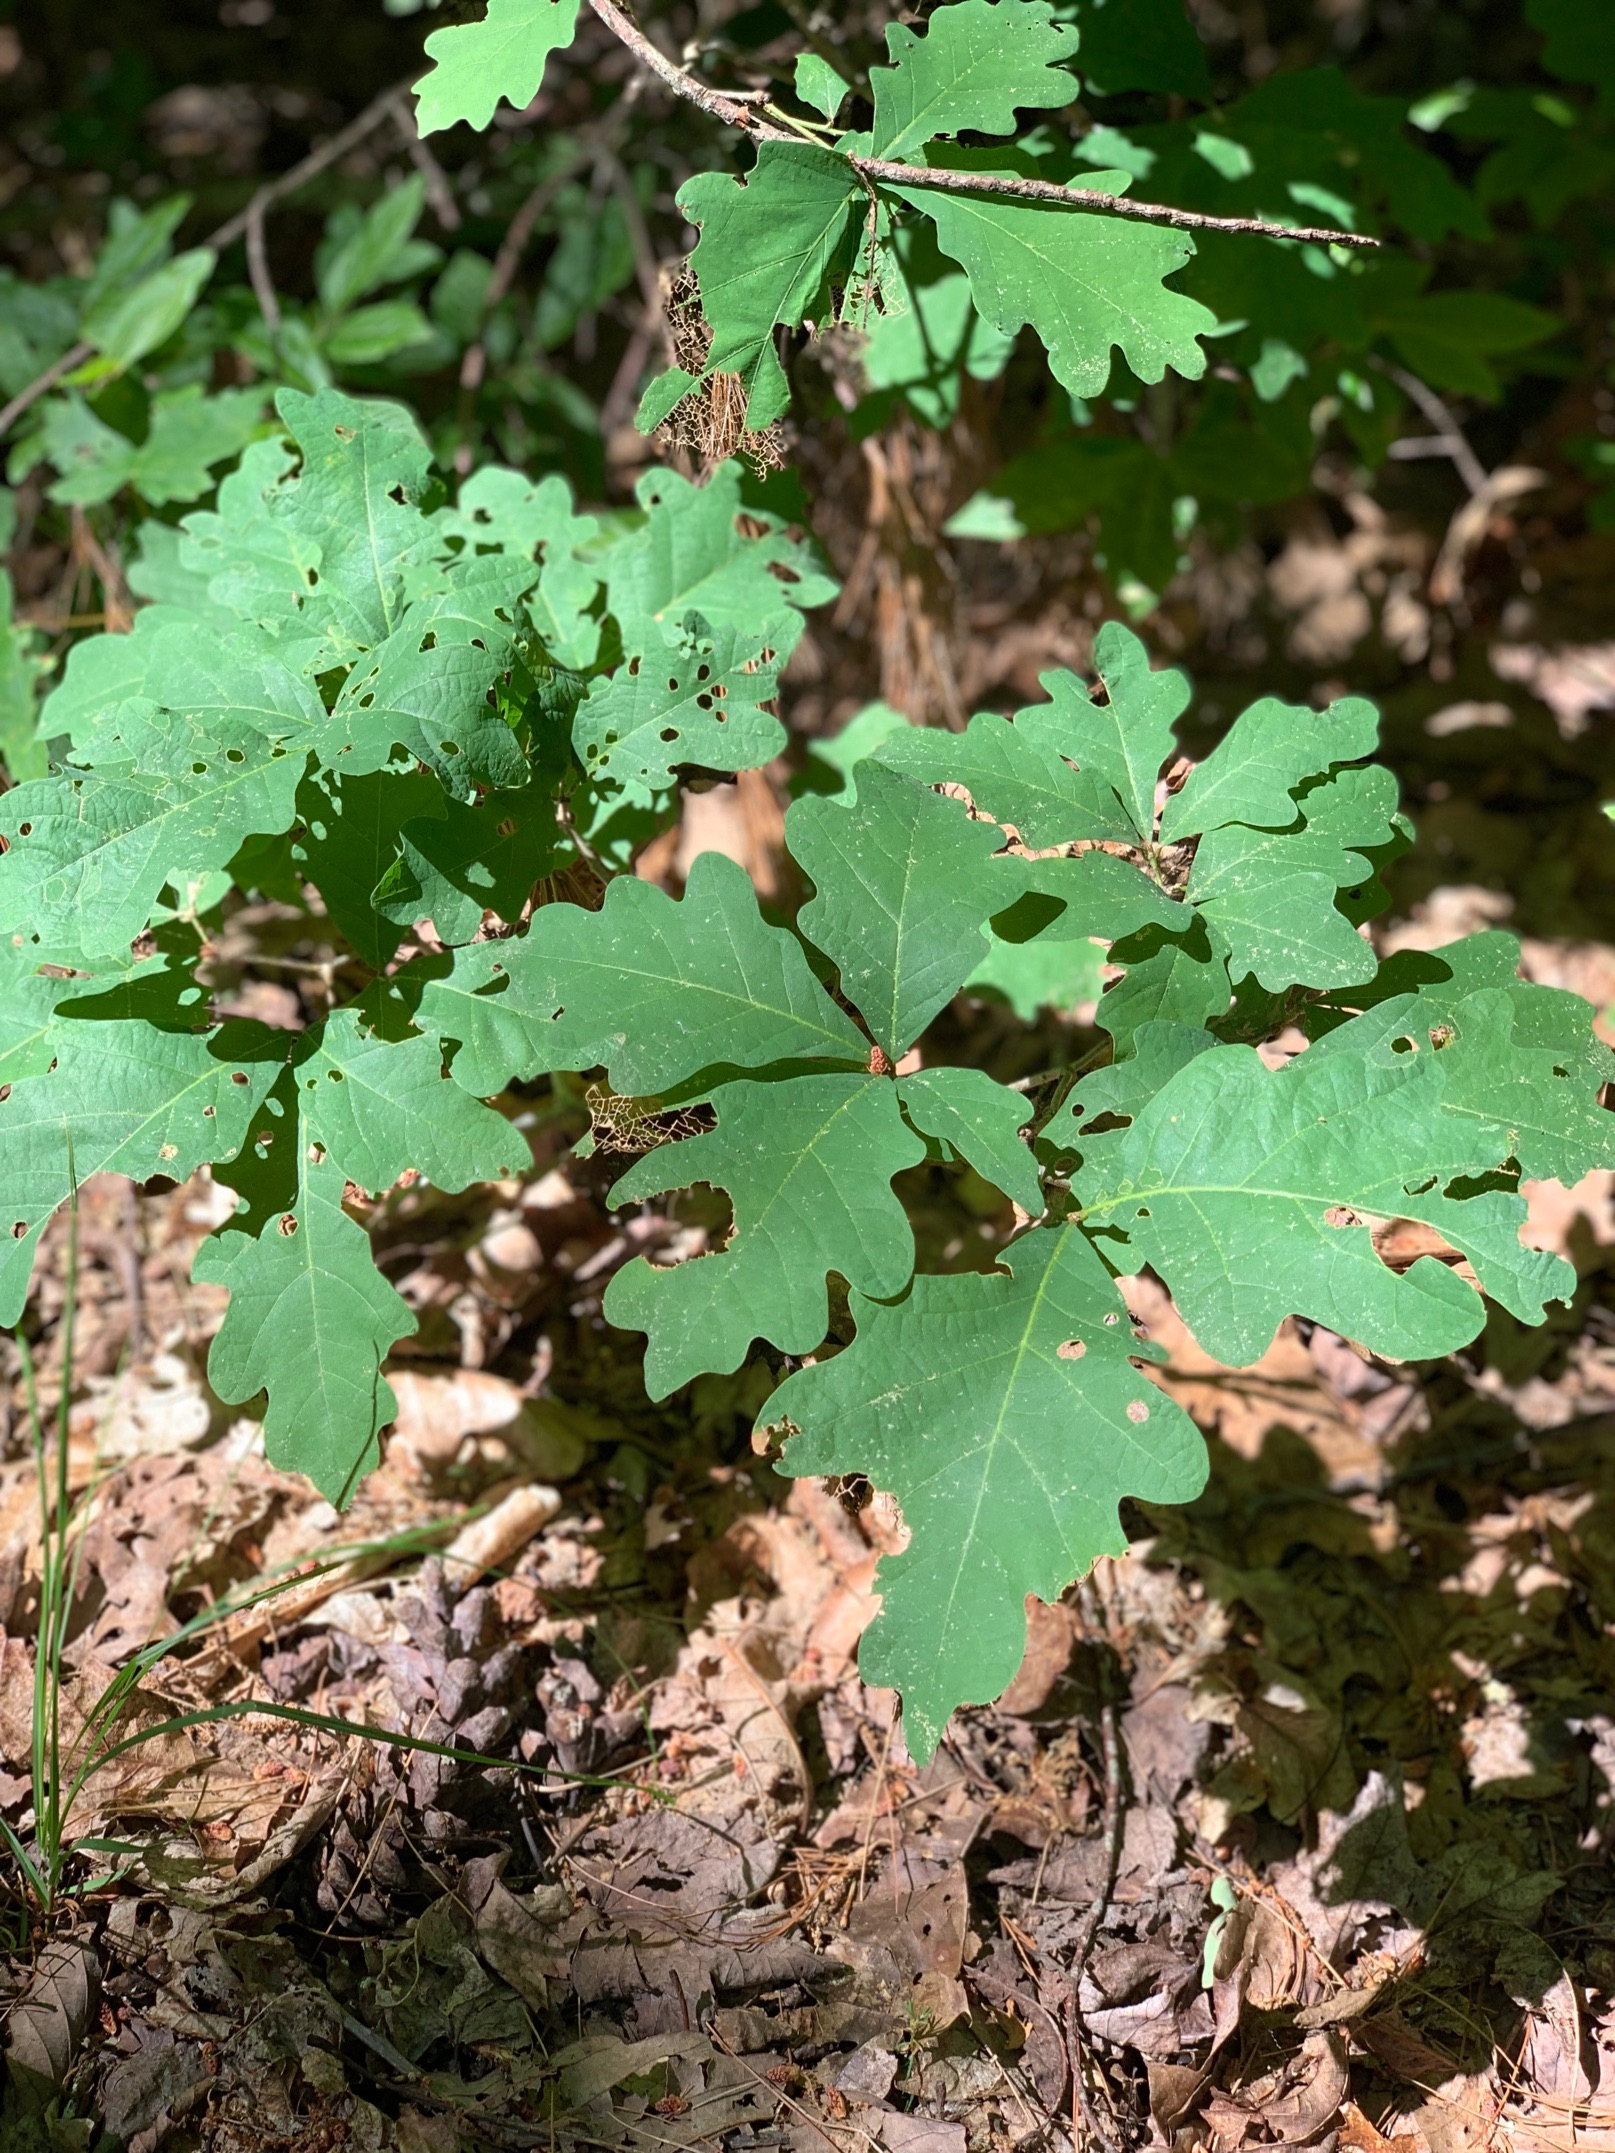
\includegraphics[width=0.5\linewidth]{english} 

}

\caption{*Quercus robur* sapling.}\label{fig:engoak}
\end{figure}

\emph{Quercus robur} is not native to North America rather it was introduced from western Asia and Europe in the 1600s as a lumber tree for furniture and shipbuilding. This tree prefers average wet and well-draining soil in full sun, but will tolerate a wide range of conditions and soil types. The lobed leaves are a rich blue-green and reddish-brown in fall. Yellow-green catkins appear with new foliage in the spring. The acorns are oblong and provide an important food source for small mammals and birds, however it could take 20 years before the tree produces acorns. (Gardenia n.d., NCSU n.d.h)

Further reading; \href{https://www.gardenia.net/plant/quercus-robur}{\emph{Quercus robur} (English Oak)}, \href{https://plants.ces.ncsu.edu/plants/quercus-robur/}{\emph{Quercus robur}}

\hypertarget{quercus-rubra}{%
\section{\texorpdfstring{\emph{Quercus rubra}}{Quercus rubra}}\label{quercus-rubra}}

\hypertarget{common-names-common-red-oak-gray-oak-eastern-red-oak-mountain-red-oak-northern-red-oak-and-red-oak}{%
\subsection{Common names; Common red oak, Gray oak, Eastern red oak, Mountain red oak, Northern red oak, and Red oak}\label{common-names-common-red-oak-gray-oak-eastern-red-oak-mountain-red-oak-northern-red-oak-and-red-oak}}

\begin{figure}

{\centering 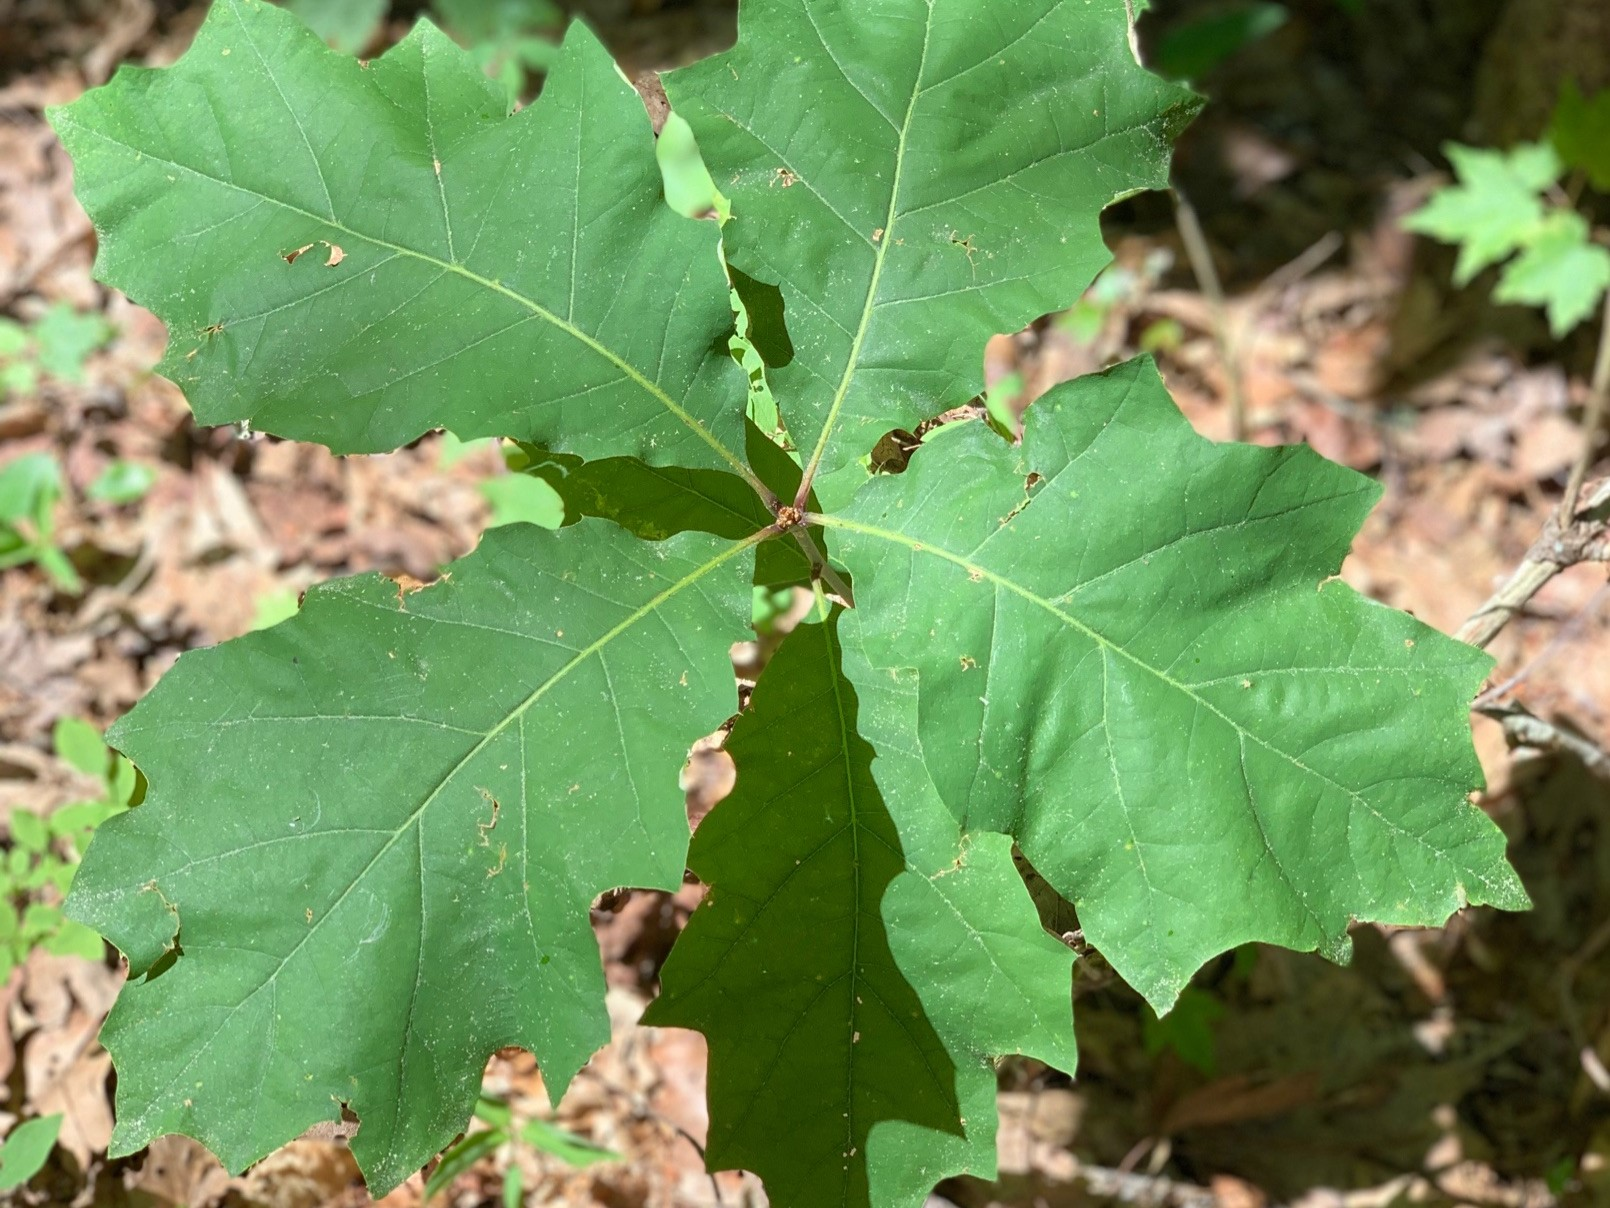
\includegraphics[width=0.5\linewidth]{redoak1} 

}

\caption{*Quercus rubra* sapling.}\label{fig:redoaks}
\end{figure}

\emph{Quercus rubra} is a deciduous tree that commonly reaches heights of 75 to 100 feet with a straight trunk and wide canopy (about 45 feet wide) on the upper 3/4ths of the tree. The bark is striped with long plates separated by deep furrows. The lobbed leaves are bristled at the tip and turn crimson, golden-orange, or russet colored in the Fall. This oak is very important lumber tree, as it is one of the fastest-growing (\textasciitilde24''/year), is easily transplanted, and endures both the cold and city conditions. This is a handsome tree for wildlife as it attracts songbirds, ground-nesting birds, butterflies, hummingbirds, and is a larval host for the Gray Hairstreak (\emph{Strymon melinus}). As new foliage begins to grow, pale yellow-green blooms are not far off, usually April to May. (Sander 1997, TWC 2013)

Further reading; \href{https://www.srs.fs.usda.gov/pubs/misc/ag_654/volume_2/quercus/rubra.htm}{Northern Red Oak}, \href{https://www.wildflower.org/plants/result.php?id_plant=quru}{\emph{Quercus rubra}}

\hypertarget{references}{%
\section*{References}\label{references}}
\addcontentsline{toc}{section}{References}

\hypertarget{refs}{}
\begin{CSLReferences}{1}{0}
\leavevmode\vadjust pre{\hypertarget{ref-gaylussacia}{}}%
\href{https://plants.ces.ncsu.edu/plants/gaylussacia-baccata/}{(n.d.a). }.

\leavevmode\vadjust pre{\hypertarget{ref-pinec2}{}}%
\href{https://www.gardenia.net/plant/pinus-echinata}{(n.d.b). }.

\leavevmode\vadjust pre{\hypertarget{ref-ACF}{}}%
ACF. 2016, April. \href{https://acf.org/}{Saving the american chestnut tree \textbar{} the american chestnut foundation}.

\leavevmode\vadjust pre{\hypertarget{ref-kal}{}}%
Figart, F. 2021, June. \href{https://www.smokiesinformation.org/news/wildflowers-101-mountain-laurel-and-rhododendron.html}{Wildflowers 101: Mountain laurel and rhododendron}.

\leavevmode\vadjust pre{\hypertarget{ref-eng2}{}}%
Gardenia. (n.d.). \href{https://www.gardenia.net/plant/quercus-robur}{Quercus robur (english oak)}.

\leavevmode\vadjust pre{\hypertarget{ref-rigida}{}}%
Gucker, C. L. 2007. \href{https://www.fs.fed.us/database/feis/plants/tree/pinrig/all.html\#Cone\%20survival\%20and\%20seedling\%20establishment:}{Pinus rigida}.

\leavevmode\vadjust pre{\hypertarget{ref-chicky}{}}%
Kuo, M. 2017, November. \href{https://www.mushroomexpert.com/laetiporus_sulphureus.html}{Laetiporus sulphureus}.

\leavevmode\vadjust pre{\hypertarget{ref-chick}{}}%
Mrs. Mushroom, J. 2022, February. \href{https://www.mushroom-appreciation.com/chicken-of-the-woods.html}{Chasing the chicken of the woods (facts, identification, and recipes) - mushroom appreciation}.

\leavevmode\vadjust pre{\hypertarget{ref-acer}{}}%
NCSU. (n.d.a). \href{https://plants.ces.ncsu.edu/plants/acer-rubrum/}{Acer rubrum (carolina maple, curled maple, red maple, scarlet maple, soft maple, swamp maple)}. Database.

\leavevmode\vadjust pre{\hypertarget{ref-castenea}{}}%
NCSU. (n.d.b). \href{https://plants.ces.ncsu.edu/plants/castanea-dentata/}{Castanea dentata (american chestnut, chestnut)}. Database.

\leavevmode\vadjust pre{\hypertarget{ref-engoak}{}}%
NCSU. (n.d.h). \href{https://plants.ces.ncsu.edu/plants/quercus-robur/}{Quercus robur (english oak, oaks, truffle oak)}. Database.

\leavevmode\vadjust pre{\hypertarget{ref-fern2}{}}%
NCSU. (n.d.f). \href{https://plants.ces.ncsu.edu/plants/onoclea-struthiopteris/}{Onoclea struthiopteris (fiddlehead fern, ostrich-feather fern, ostrich fern, shuttlecock fern)}.

\leavevmode\vadjust pre{\hypertarget{ref-iris}{}}%
NCSU. (n.d.c). \href{https://plants.ces.ncsu.edu/plants/iris-sanguinea/}{Iris sanguinea (japanese iris, siberian iris)}. Database.

\leavevmode\vadjust pre{\hypertarget{ref-kal2}{}}%
NCSU. (n.d.d). \href{https://plants.ces.ncsu.edu/plants/kalmia-latifolia/}{Kalmia latifolia (calico bush, ivy bush, laurel, mountain ivy, mountain laurel, sheepkill, spoonwood)}. Database.

\leavevmode\vadjust pre{\hypertarget{ref-pinec}{}}%
NCSU. (n.d.g). \href{https://plants.ces.ncsu.edu/plants/pinus-echinata/}{Pinus echinata (old-field pine, rosemary pine, short-leaf pine, shortleaf pine, yellow pine)}. Database.

\leavevmode\vadjust pre{\hypertarget{ref-tulip}{}}%
NCSU. (n.d.e). \href{https://plants.ces.ncsu.edu/plants/liriodendron-tulipifera/}{Liriodendron tulipifera (tulip poplar, tulip tree, yellow poplar, yellow-poplar)}.

\leavevmode\vadjust pre{\hypertarget{ref-chick3}{}}%
O'Reilly, P., and S. Parker. (n.d.). \href{https://www.first-nature.com/fungi/laetiporus-sulphureus.php}{Laetiporus sulphureus, chicken-of-the-woods, identification}.

\leavevmode\vadjust pre{\hypertarget{ref-iris2}{}}%
PFAF. (n.d.). \href{https://pfaf.org/user/Plant.aspx?LatinName=Iris+sanguinea}{Iris sanguinea blood iris}. Database.

\leavevmode\vadjust pre{\hypertarget{ref-galax}{}}%
Predny, M. L., and J. L. Chamberlain. 2005. \href{https://www.srs.fs.usda.gov/pubs/gtr/gtr_srs087.pdf}{Galax (galax urceolata): An annotated bibliography}. U.S. Department of Agriculture, Forest Service, Southern Research Station.

\leavevmode\vadjust pre{\hypertarget{ref-red2}{}}%
Sander, I. L. 1997, October. \href{https://www.srs.fs.usda.gov/pubs/misc/ag_654/volume_2/quercus/rubra.htm}{Northern red oak}.

\leavevmode\vadjust pre{\hypertarget{ref-redoak}{}}%
TWC. 2013, June. \href{https://www.wildflower.org/plants/result.php?id_plant=quru}{Quercus rubra (northern red oak)}. Database.

\leavevmode\vadjust pre{\hypertarget{ref-fern}{}}%
TWC. 2017b, July. \href{https://www.wildflower.org/plants/result.php?id_plant=MAST}{Matteuccia struthiopteris (ostrich fern)}. Database.

\leavevmode\vadjust pre{\hypertarget{ref-kal3}{}}%
TWC. 2017a, July. \href{https://www.wildflower.org/plants/result.php?id_plant=KALA}{Kalmia latifolia (mountain laurel)}.

\leavevmode\vadjust pre{\hypertarget{ref-tulip2}{}}%
TWC. 2021, May. \href{https://www.wildflower.org/plants/result.php?id_plant=LITU}{Liriodendron tulipifera (tulip tree)}.

\leavevmode\vadjust pre{\hypertarget{ref-acer2}{}}%
TWC, and GDG. 2015, November. \href{https://www.wildflower.org/plants/result.php?id_plant=acru}{Acer rubrum (red maple)}.

\leavevmode\vadjust pre{\hypertarget{ref-uniflora}{}}%
\href{https://www.fs.fed.us/wildflowers/beauty/mycotrophic/monotropa_uniflora.shtml}{USFS. (n.d.). }.

\leavevmode\vadjust pre{\hypertarget{ref-snail}{}}%
Wikipedia. 2021, March. \href{https://en.wikipedia.org/w/index.php?title=Patera_clarki_nantahala\&oldid=1010217193}{Patera clarki nantahala}.

\end{CSLReferences}

\end{document}
